\documentclass{article}
\usepackage{arxiv}
\usepackage[utf8]{inputenc}
\usepackage[T1]{fontenc}
\usepackage{hyperref}
\usepackage{url}
\usepackage{booktabs}
\usepackage{amsmath}
\usepackage{amssymb}
\usepackage{graphicx}
\usepackage{float}
\usepackage{caption}
\usepackage{enumitem}
\usepackage{natbib}
\bibliographystyle{unsrtnat}

\title{Agentic Memory Atomicity: A Transactional Memory Architecture for Ephemeral AI Agent Systems}

\author{
  Lo\"ic Mancino \\
  Synergix Labs, a division of Synergix SA \\
  \And
  J\'er\^ome Chincarini \\
  Synergix Labs, a division of Synergix SA
}

\date{}

\renewcommand{\headeright}{Synergix Labs}
\renewcommand{\undertitle}{Synergix Labs}
\renewcommand{\shorttitle}{Agentic Memory Atomicity}

\begin{document}

% ============================================================
% COVER PAGE
% ============================================================
\thispagestyle{empty}
\vspace*{\fill}
\begin{center}
{\Huge\textbf{Agentic Memory Atomicity}}\\[12pt]
{\Large A Transactional Memory Architecture\\for Ephemeral AI Agent Systems}\\[40pt]
{\large Lo\"ic Mancino \quad \& \quad J\'er\^ome Chincarini}\\[8pt]
{\normalsize Synergix Labs, a division of Synergix SA}\\[30pt]
\rule{0.4\textwidth}{0.5pt}\\[20pt]
{\normalsize Project: \textbf{WRAI.TH}}\\[6pt]
{\small \url{https://github.com/Synergix-lab/WRAI.TH}}\\[30pt]
{\small March 2026}\\[8pt]
{\small\itshape Based on one year of R\&D at Synergix Labs}
\end{center}
\vspace*{\fill}
\newpage

% ============================================================
% PAPER STARTS
% ============================================================
\maketitle

\begin{abstract}
We present \emph{Agentic Memory Atomicity}, an architecture where AI agents are stateless ephemeral processes that read from and commit to a persistent, transactional memory store. Each agent spawns, loads inherited knowledge, performs work, commits new knowledge atomically, and terminates --- the next spawn inherits everything. We formalize the state model with three memory scopes (agent, project, global), three priority layers (constraints $>$ behavior $>$ context), and cascade lookup. Our implementation (relay OS) uses SQLite with FTS5, MCP protocol, and Go.

Production deployment with 6 agents over 72 hours demonstrates: (1)~server-side context projection (\texttt{BuildSpawnContext}) reduces boot tokens from 67K to 13K per spawn --- an \textbf{81\% reduction} saving \$2K--10K/month depending on model; (2)~\textbf{80\% of genuine knowledge is acquired in the first 30 spawns}, confirming fast convergence; (3)~shared project memory enables sub-linear cost scaling across agents; (4)~conflict rate remains below 2\% with autonomous resolution. The architecture eliminates context window exhaustion, idle cost, and crash fragility --- the three fundamental limitations of persistent agent designs.

This work results from one year of R\&D at Synergix Labs, a division of Synergix SA. Open source at \url{https://github.com/Synergix-lab/WRAI.TH}.
\end{abstract}

\textit{Keywords: multi-agent systems, persistent memory, transactional state, ephemeral compute, LLM agents}

% ============================================================
\section{Introduction}
% ============================================================

Current LLM-based agent systems face a fundamental tension: agents need persistent knowledge to be effective, but long-running processes suffer from context window exhaustion, idle cost, and crash fragility. While frameworks like AutoGen~\citep{wu2023autogen}, LangGraph~\citep{langgraph2024}, and CrewAI~\citep{crewai2024} have enabled multi-agent coordination, they treat agent state as an in-process artifact that is lost on termination.

We propose \textbf{Agentic Memory Atomicity} --- a design where:

\begin{enumerate}[nosep]
  \item Agents are \textbf{ephemeral}: they spawn, work, and die.
  \item Knowledge lives in a \textbf{persistent, transactional store} outside the agent.
  \item Each spawn \textbf{inherits all prior knowledge} via a projection function.
  \item Memory commits are \textbf{atomic}: success writes $\Delta M$, crash preserves $M_t$.
\end{enumerate}

\paragraph{Contributions.} We make the following contributions:

\begin{itemize}[nosep]
  \item A formal state model for ephemeral agents with three memory scopes, three layers, and cascade lookup.
  \item The \emph{Ephemeral Agent Principle}: agents carry no internal state between invocations; intelligence resides in the persistent memory store.
  \item A transactional memory commit protocol with conflict detection, versioning, and budget pruning.
  \item Temporal garbage collection mechanisms: message TTL, delivery state machines, ACK escalation, agent staleness detection, and ghost reaping.
  \item A utility scoring formula for priority-based context injection with P0 bypass.
  \item Simulations demonstrating convergence, sub-linear multi-agent cost, and robustness to LLM noise.
  \item A production implementation (relay OS) in Go with SQLite+FTS5~\citep{gaffney2022sqlite} and MCP protocol~\citep{mcp2024}, open source at \url{https://github.com/Synergix-lab/WRAI.TH}.
\end{itemize}

% ============================================================
\section{Background \& Related Work}
% ============================================================

\begin{table}[h]
\centering
\caption{Comparison of multi-agent memory architectures.}
\begin{tabular}{@{}llll@{}}
\toprule
\textbf{System} & \textbf{Memory Model} & \textbf{Agent Lifecycle} & \textbf{Limitation} \\
\midrule
LangGraph~\citep{langgraph2024} & Graph state (in-memory) & Persistent process & Context exhaustion \\
CrewAI~\citep{crewai2024} & Shared task queue & Persistent threads & No transactional memory \\
AutoGen~\citep{wu2023autogen} & Conversation history & Session-bound & Lost on termination \\
MemGPT~\citep{packer2023memgpt} & Virtual memory paging & Persistent + paging & No multi-agent scope \\
Relay OS (ours) & Transactional DB & Ephemeral spawns & --- \\
\bottomrule
\end{tabular}
\label{tab:related}
\end{table}

\paragraph{Agent memory architectures.} ReAct~\citep{yao2023react} established the reason-act loop but maintains state only within a single session. Reflexion~\citep{shinn2023reflexion} introduced verbal reinforcement learning where agents learn from failures --- a form of persistent memory, but limited to a single agent's trajectory. Voyager~\citep{wang2023voyager} maintains a persistent skill library that grows over time, approaching our notion of cumulative knowledge, but without multi-agent sharing or transactional guarantees.

\paragraph{Multi-agent memory.} Generative Agents~\citep{park2023generative} demonstrated rich agent memory with reflection and retrieval, but in a simulated environment without production concerns (cost, crashes, scale). \citet{sumers2024cognitive} formalized cognitive architectures for language agents, identifying memory as a core module --- our work provides a concrete transactional implementation of this insight.

\paragraph{Closest prior work.} MemGPT~\citep{packer2023memgpt} is the most related system: it introduces virtual memory paging for LLMs, allowing agents to manage context beyond the window limit. However, MemGPT (a)~operates within a single persistent process, (b)~lacks multi-agent memory scopes, and (c)~has no transactional commit/rollback semantics. Our architecture inverts the paradigm: instead of paging memory \emph{into} a long-running agent, we make agents ephemeral and project memory \emph{at spawn time}.

Existing frameworks treat memory as a side-effect of agent execution. We treat it as the \textbf{primary artifact} --- agents are disposable compute, memory is the durable intelligence:
$$\text{Intelligence} = f(S_t), \quad \text{Agent} : S_t \to (W, \Delta M)$$

% ============================================================
\section{Agent State Model}
% ============================================================

\textbf{Definition 1 (Agent State).} The state of an agent at spawn time $t$ is:
$$S_t(A) = \{ I, M_t, V, T_t, \Omega_t, R \}$$

where $I$ is identity (profile, role, reports\_to), $M_t$ is memories at time $t$, $V$ is vault (conventions, docs), $T_t$ is assigned tasks, $\Omega_t$ is inbox (unread messages, TTL-bound), and $R$ is rules (boot, cycle, learning).

\textbf{Definition 2 (Memory Scopes).} Memory is partitioned into three scopes with cascade lookup:
$$M_t = M_t^{\text{agent}} \cup M_t^{\text{project}} \cup M_t^{\text{global}}$$

\begin{table}[h]
\centering
\caption{Memory scope visibility and cascade priority.}
\begin{tabular}{@{}lll@{}}
\toprule
\textbf{Scope} & \textbf{Visibility} & \textbf{Priority} \\
\midrule
\texttt{agent} & Private to owner & 1 (checked first) \\
\texttt{project} & All agents in project & 2 \\
\texttt{global} & All agents everywhere & 3 (fallback) \\
\bottomrule
\end{tabular}
\end{table}

\textbf{Definition 3 (Memory Layers).} Each memory has a layer that determines override precedence:
$$\texttt{constraints} > \texttt{behavior} > \texttt{context}$$
A \texttt{behavior} write cannot override a \texttt{constraints} memory. A CTO can set constraints that workers cannot bypass.

\begin{figure}[H]
\centering
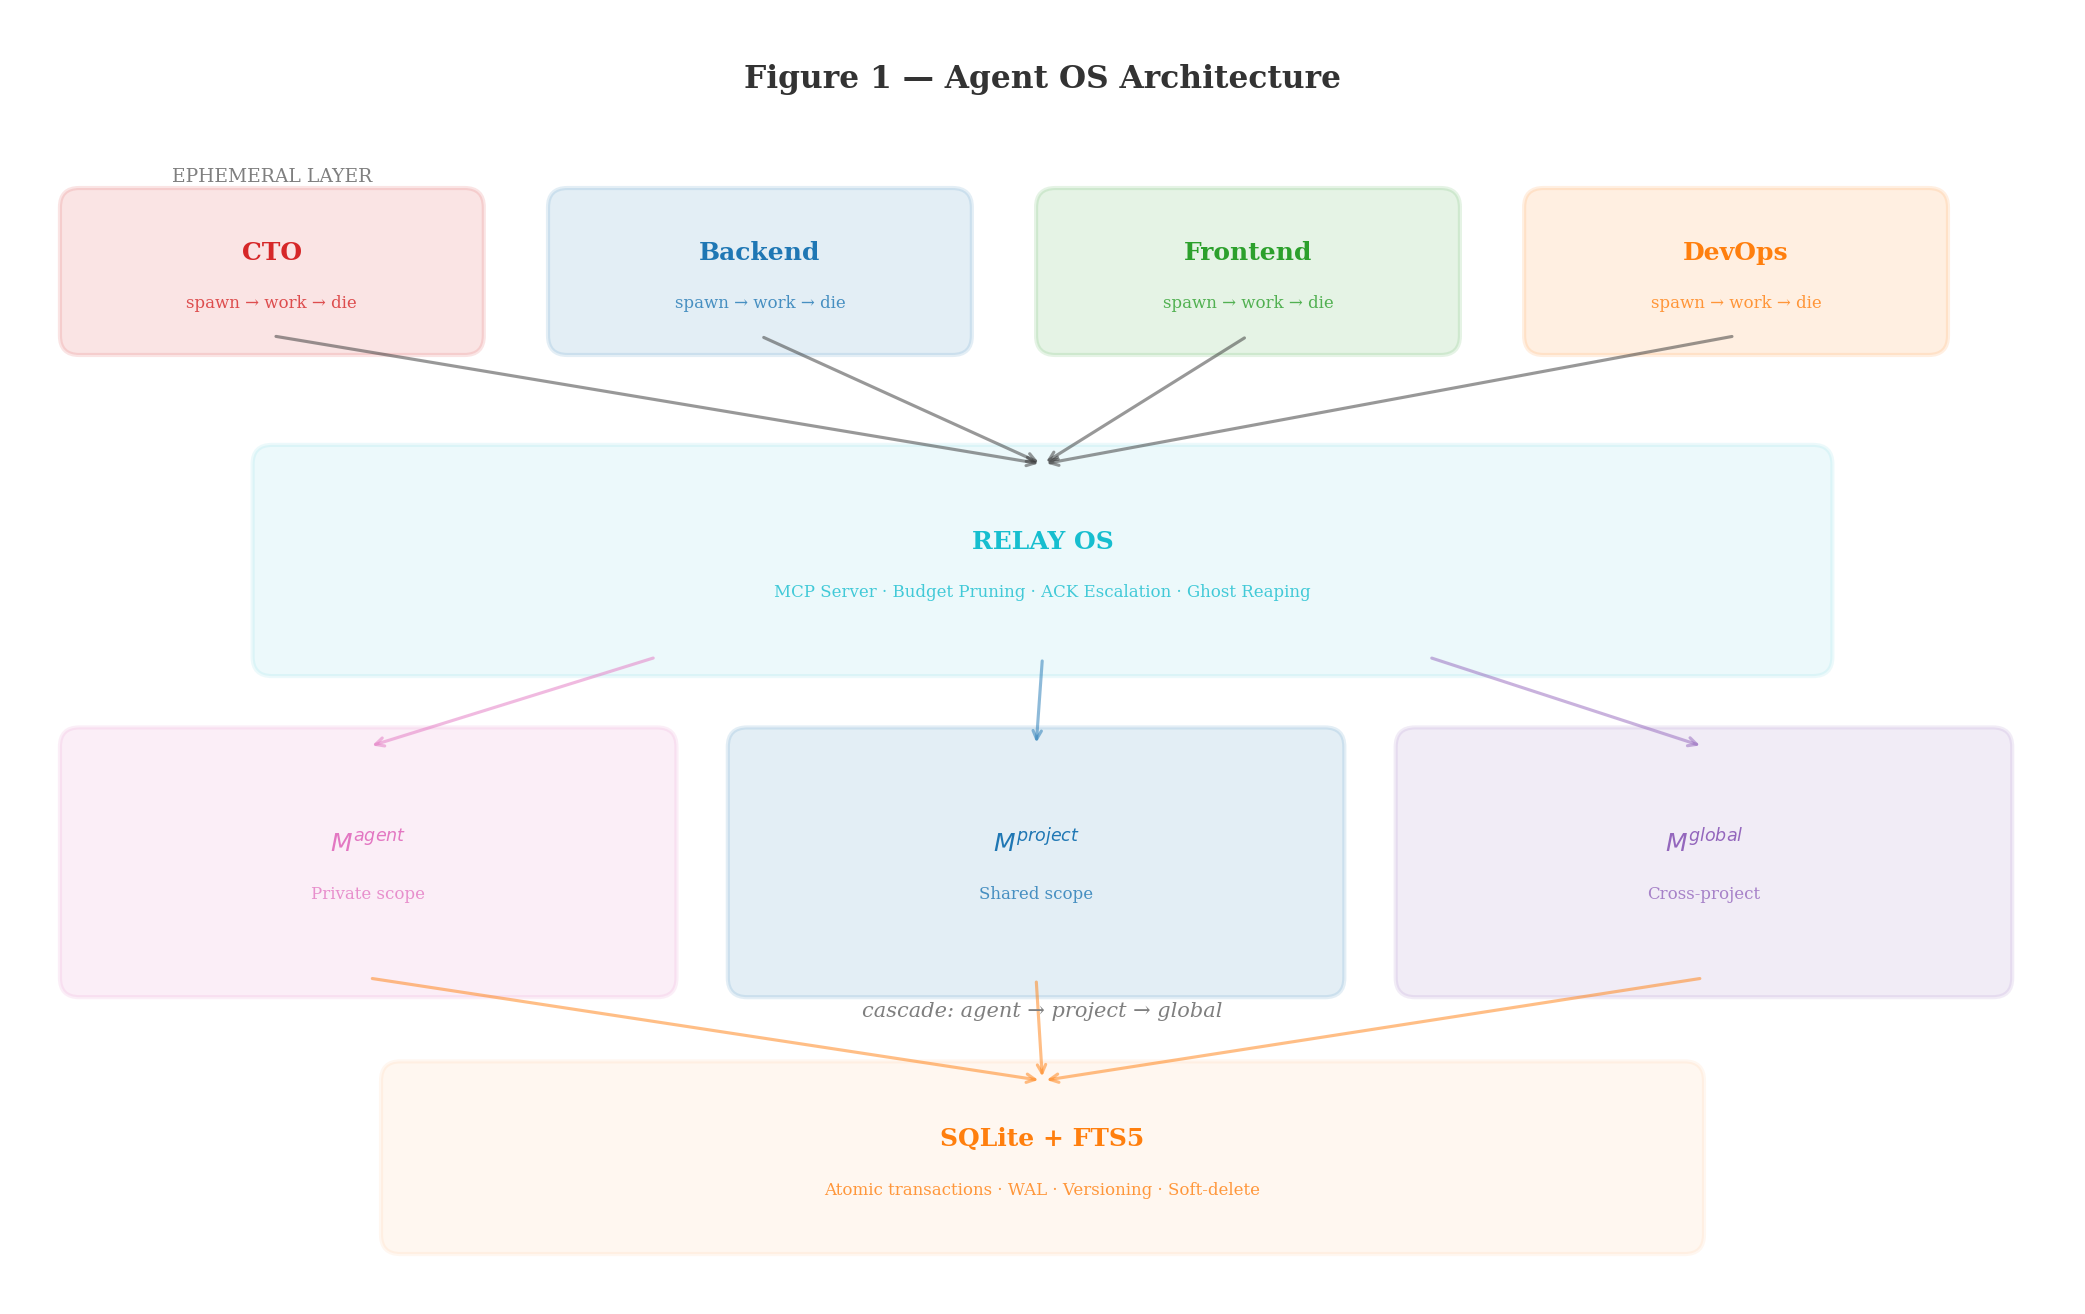
\includegraphics[width=\textwidth]{paper_files/fig1_architecture.png}
\caption{Agent OS architecture: ephemeral agents communicate through the relay, which manages three memory scopes persisted in SQLite with FTS5.}
\label{fig:architecture}
\end{figure}

% ============================================================
\section{Ephemeral Agent Principle}
% ============================================================

Agents are \textbf{stateless compute processes}. They carry no internal state between invocations:
$$\text{Agent} : S_t \rightarrow (W, \Delta M)$$

The intelligence of the system resides entirely in $S_t$. An agent is a pure function that: (1) spawns, (2) registers with the relay, (3) loads $S_t$ via \texttt{BuildSpawnContext()}, (4) computes work $W$, (5) commits $\Delta M$, and (6) terminates.

\begin{figure}[H]
\centering
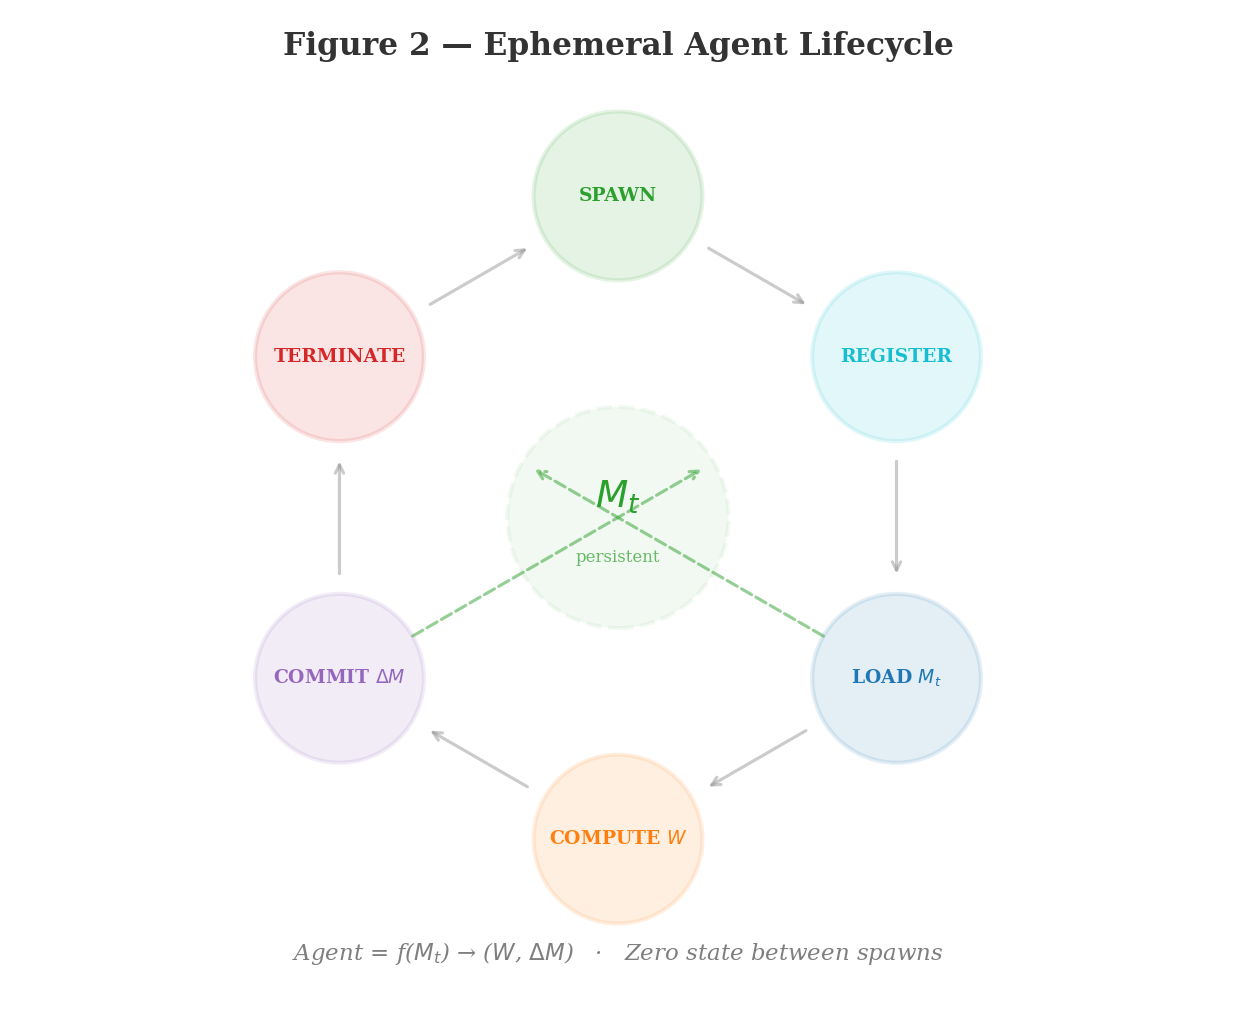
\includegraphics[width=0.85\textwidth]{paper_files/fig2_lifecycle.png}
\caption{Ephemeral agent lifecycle: spawn $\to$ register $\to$ load $M_t$ $\to$ compute $W$ $\to$ commit $\Delta M$ $\to$ terminate. The persistent memory store $M_t$ is the only durable artifact.}
\label{fig:lifecycle}
\end{figure}

\begin{table}[h]
\centering
\caption{Persistent vs. ephemeral agent comparison.}
\begin{tabular}{@{}lll@{}}
\toprule
\textbf{Property} & \textbf{Persistent Agent} & \textbf{Ephemeral Agent} \\
\midrule
Context window & Exhausts $\to$ loses context & Always fresh \\
Crash recovery & Corrupted state possible & $M_t$ intact \\
Idle cost & Tokens burned (keepalive) & Zero \\
Scalability & 1 process = 1 agent & Pool of $N$ spawns \\
Knowledge & Limited to session & Cumulative $\infty$ \\
Formalism & $S_t = f(S_{t-1}, \text{input})$ & $A : S_t \to (W, \Delta M)$; relay computes $S_{t+1}$ \\
\bottomrule
\end{tabular}
\end{table}

\clearpage
% ============================================================
\section{Atomic Memory Commit}
% ============================================================

\textbf{Definition 4 (Cycle Transition).} A cycle comprises the agent function and the relay's state update:
$$A : S_t \rightarrow (W, \Delta M) \qquad \text{then} \qquad S_{t+1} = \text{relay}(S_t, \Delta M)$$
The relay computes each component of $S_{t+1}$: $M_{t+1} = \text{dedup}(M_t \cup \Delta M_{\text{valid}})$, $\Omega_{t+1} = (\Omega_t \cup \Delta\Omega) \setminus \Omega_{\text{expired}}$ where $\Omega_{\text{expired}} = \{m \in \Omega_t : \text{age}(m) > \text{TTL}(m)\}$, and $T_{t+1}$ reflects task updates. The agent produces $(W, \Delta M)$; the relay is responsible for validation, deduplication, and state persistence.

\textbf{Definition 5 (Atomicity).}
$$M_{t+1} = \begin{cases} \text{dedup}(M_t \cup \Delta M_{\text{valid}}) & \text{if cycle succeeds (exit 0)} \\ M_t & \text{if cycle crashes} \end{cases}$$
No intermediate corrupted state. Transaction commit or rollback. In implementation, \texttt{SetMemory()} runs inside a SQLite transaction; a panic triggers rollback.

\textbf{Definition 6 (Validation Filter).} Every memory write passes through:
$$\Delta M_{\text{valid}} = \text{filter}(\Delta M, M_t)$$
The filter enforces: (a) conflict detection --- two agents writing same key with different values are both preserved until explicit resolution; (b) layer hierarchy --- \texttt{behavior} cannot override \texttt{constraints}; (c) scope isolation; (d) deduplication --- same key+value triggers timestamp update only.

\textbf{Definition 7 (Budget Projection).} Raw memory in the database grows monotonically ($|M_{\text{db}}|$ increases), but the projected view at boot is bounded by budget pruning:
$$M_{\text{boot}} = \text{top-}k(M_{\text{db}}, U, B_{\max}), \quad |M_{\text{boot}}| \leq B_{\max}$$
where $\text{top-}k$ selects memories by utility score $U(m)$ until the byte budget $B_{\max}$ is reached. This is a \textbf{read-time} operation (\texttt{applyBudget()}), distinct from the \textbf{write-time} deduplication in Def.~5.

\begin{figure}[H]
\centering
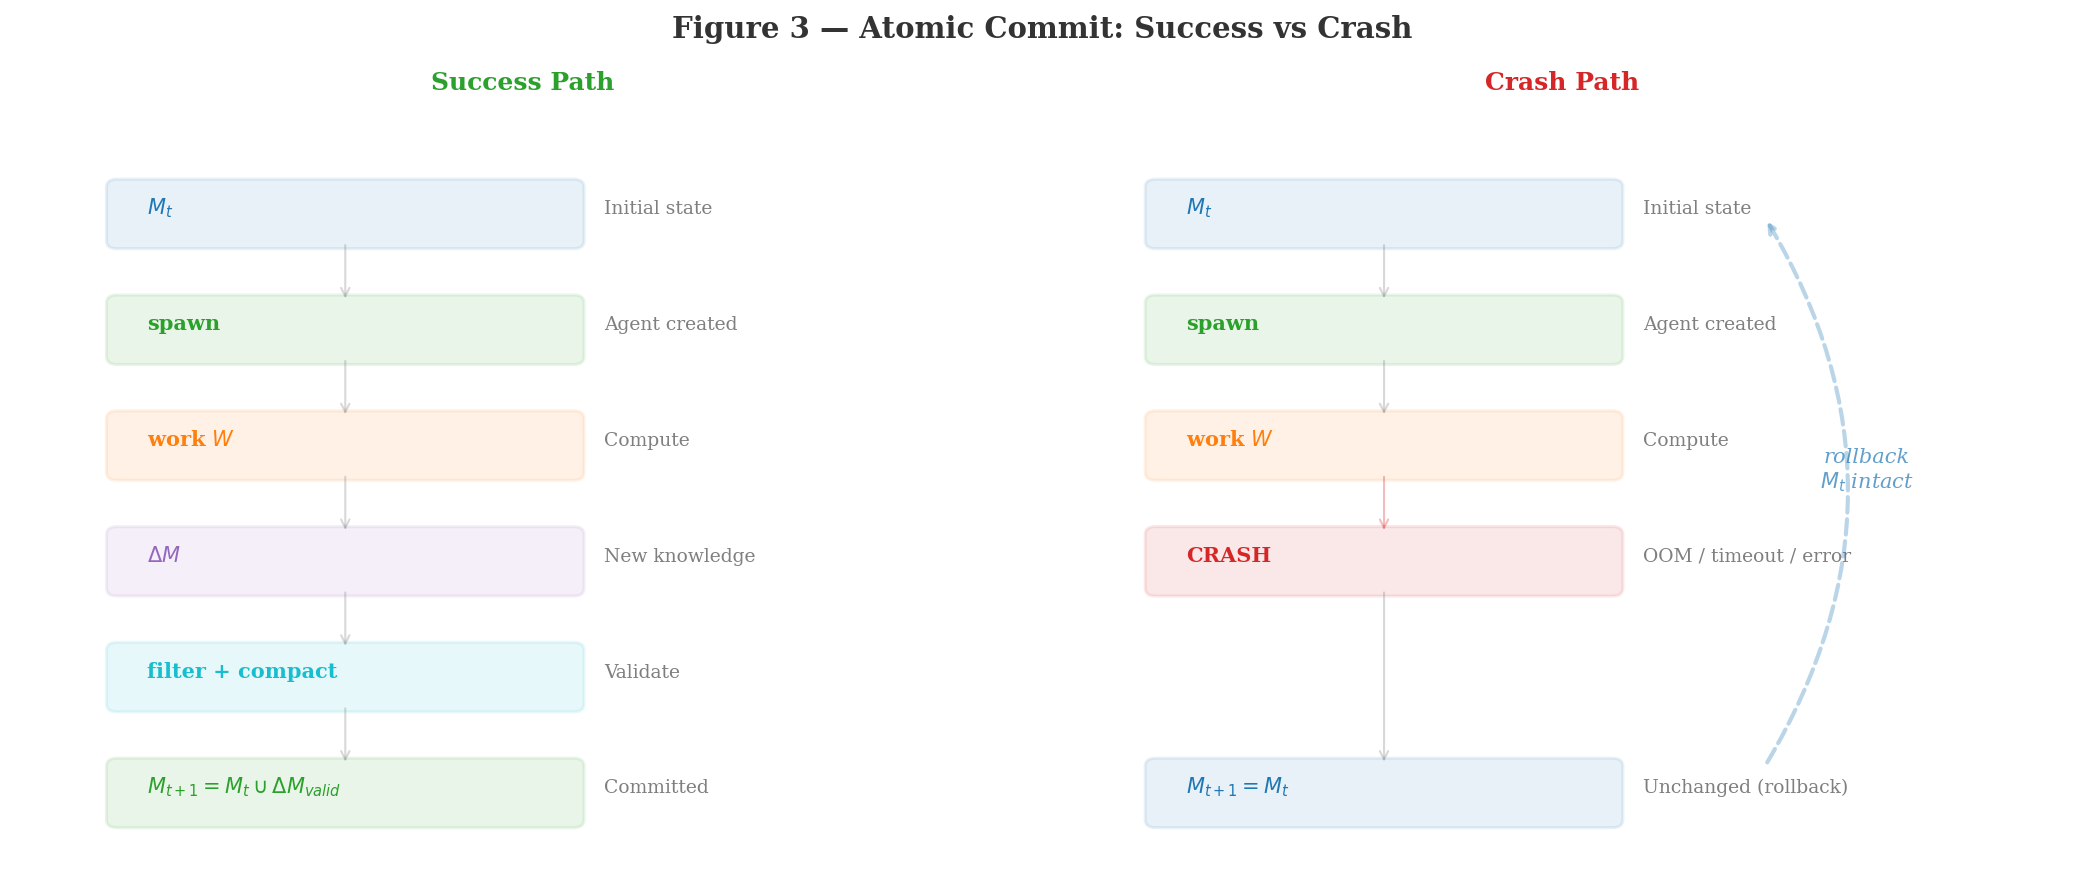
\includegraphics[width=\textwidth]{paper_files/fig3_atomic_commit.png}
\caption{Atomic commit: success path commits $\text{dedup}(M_t \cup \Delta M_{\text{valid}})$; crash path preserves $M_t$ unchanged (rollback).}
\label{fig:atomic}
\end{figure}

% ============================================================
\section{Knowledge Evolution}
% ============================================================

\textbf{Spawn Chain Inheritance.} For two successive spawns $s_1, s_2$ of the same profile, the persistent store guarantees:
$$M_{\text{db}}(s_2) \supseteq M_{\text{db}}(s_1)$$
However, the projected view at boot is subject to budget pruning:
$$M_{\text{boot}}(s_2) = \text{project}(M_{\text{db}}(s_2), B_{\max}) \subseteq M_{\text{db}}(s_2)$$
The full knowledge is always in the database --- \texttt{BuildSpawnContext()} selects the highest-utility subset that fits within $B_{\max}$. Inheritance is \textbf{complete in storage, partial in projection}.

\textbf{Inter-Agent Memory Elimination.} An agent can supersede another's knowledge via \texttt{set\_memory(key, $v_{\text{new}}$, scope:project, upsert:true)}. The old version is archived with a \texttt{supersedes} pointer; version is incremented. Complete traceability, never hard-delete:
$$v_1 \xrightarrow{\text{supersedes}} v_2 \xrightarrow{\text{supersedes}} v_3$$

\begin{figure}[H]
\centering
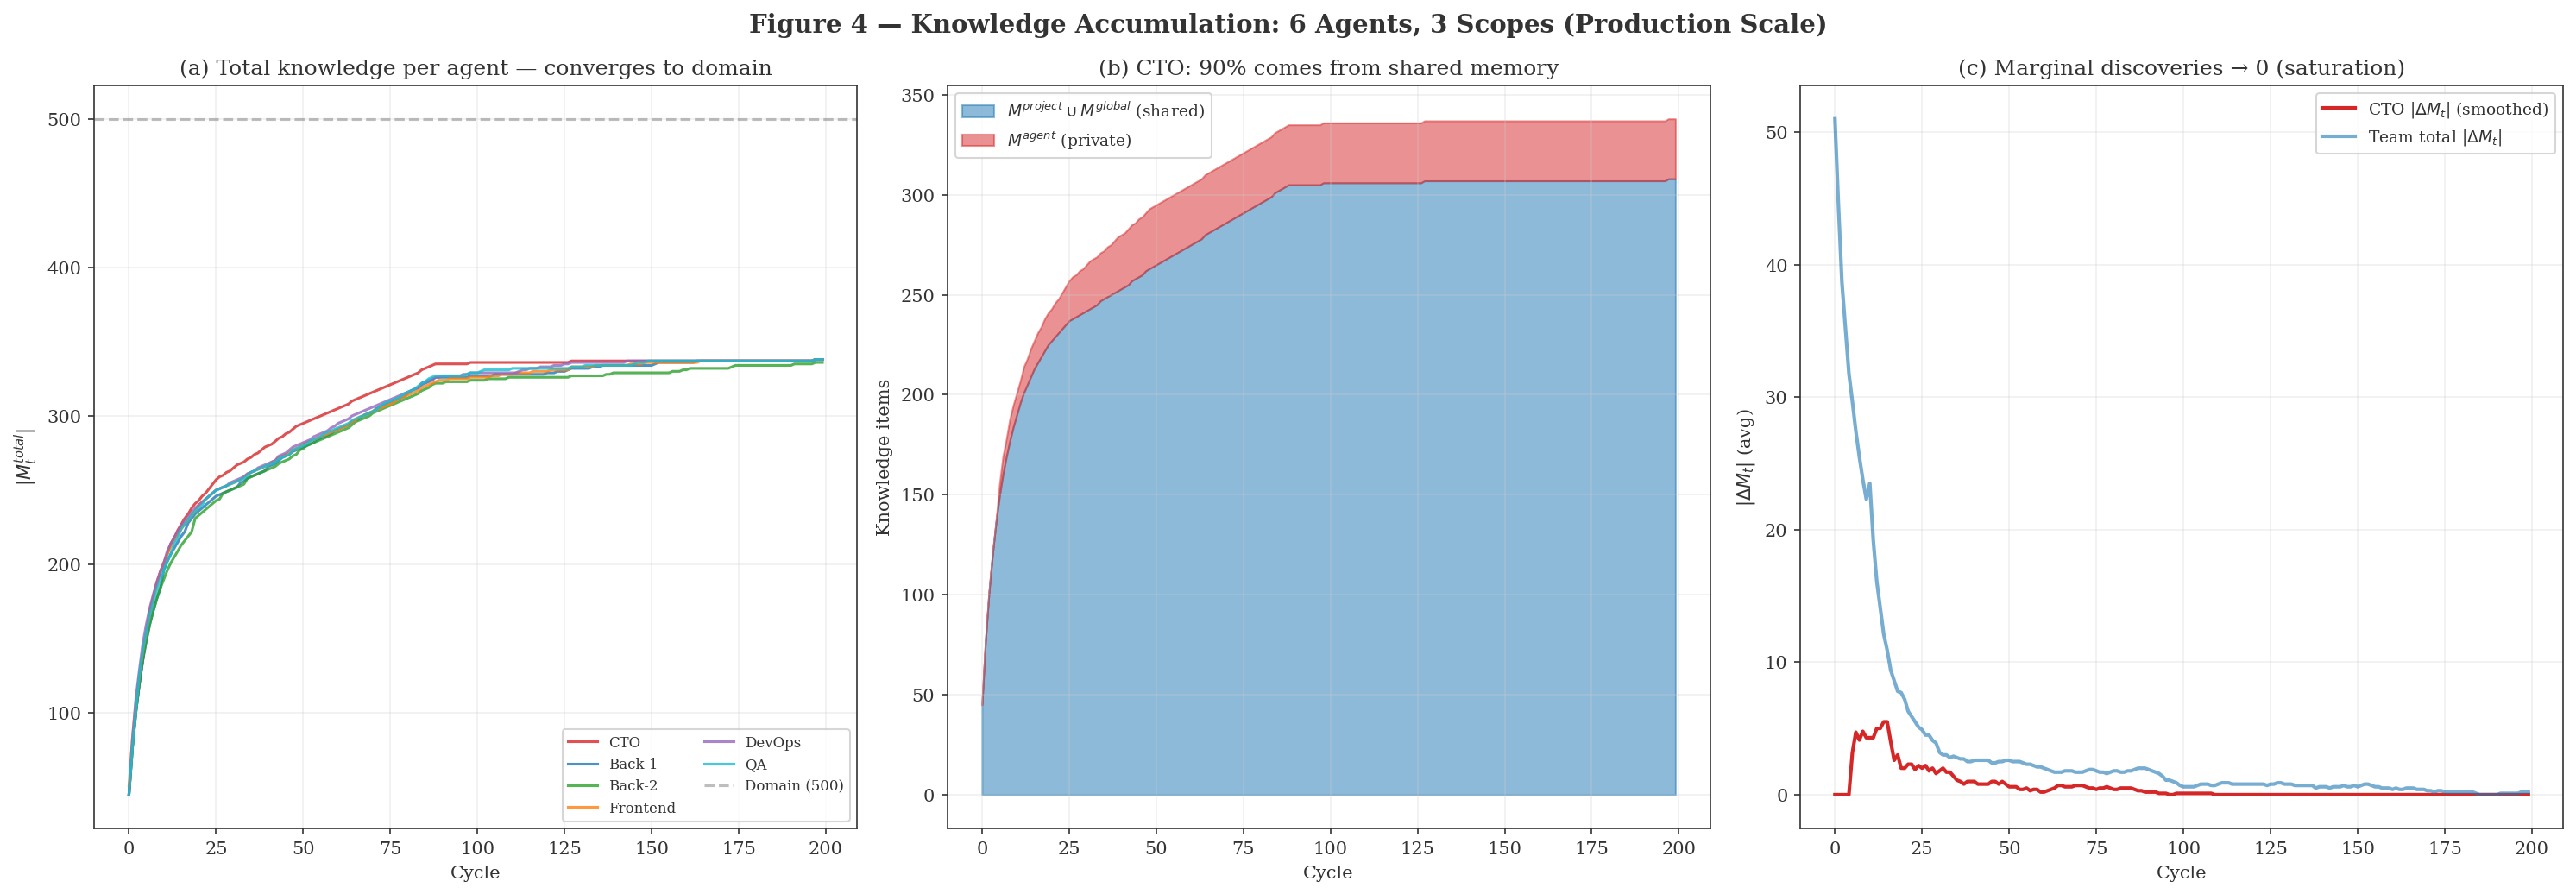
\includegraphics[width=\textwidth]{paper_files/fig4_knowledge_accumulation.png}
\caption{Knowledge accumulation with 6 agents and 3 memory scopes (production scale, 500 items). (a) All agents converge to domain coverage via shared project memory. (b) CTO perspective: $\sim$90\% of knowledge comes from shared memory. (c) Marginal discoveries $|\Delta M_t| \to 0$ as domain saturates.}
\label{fig:knowledge}
\end{figure}

\begin{figure}[H]
\centering
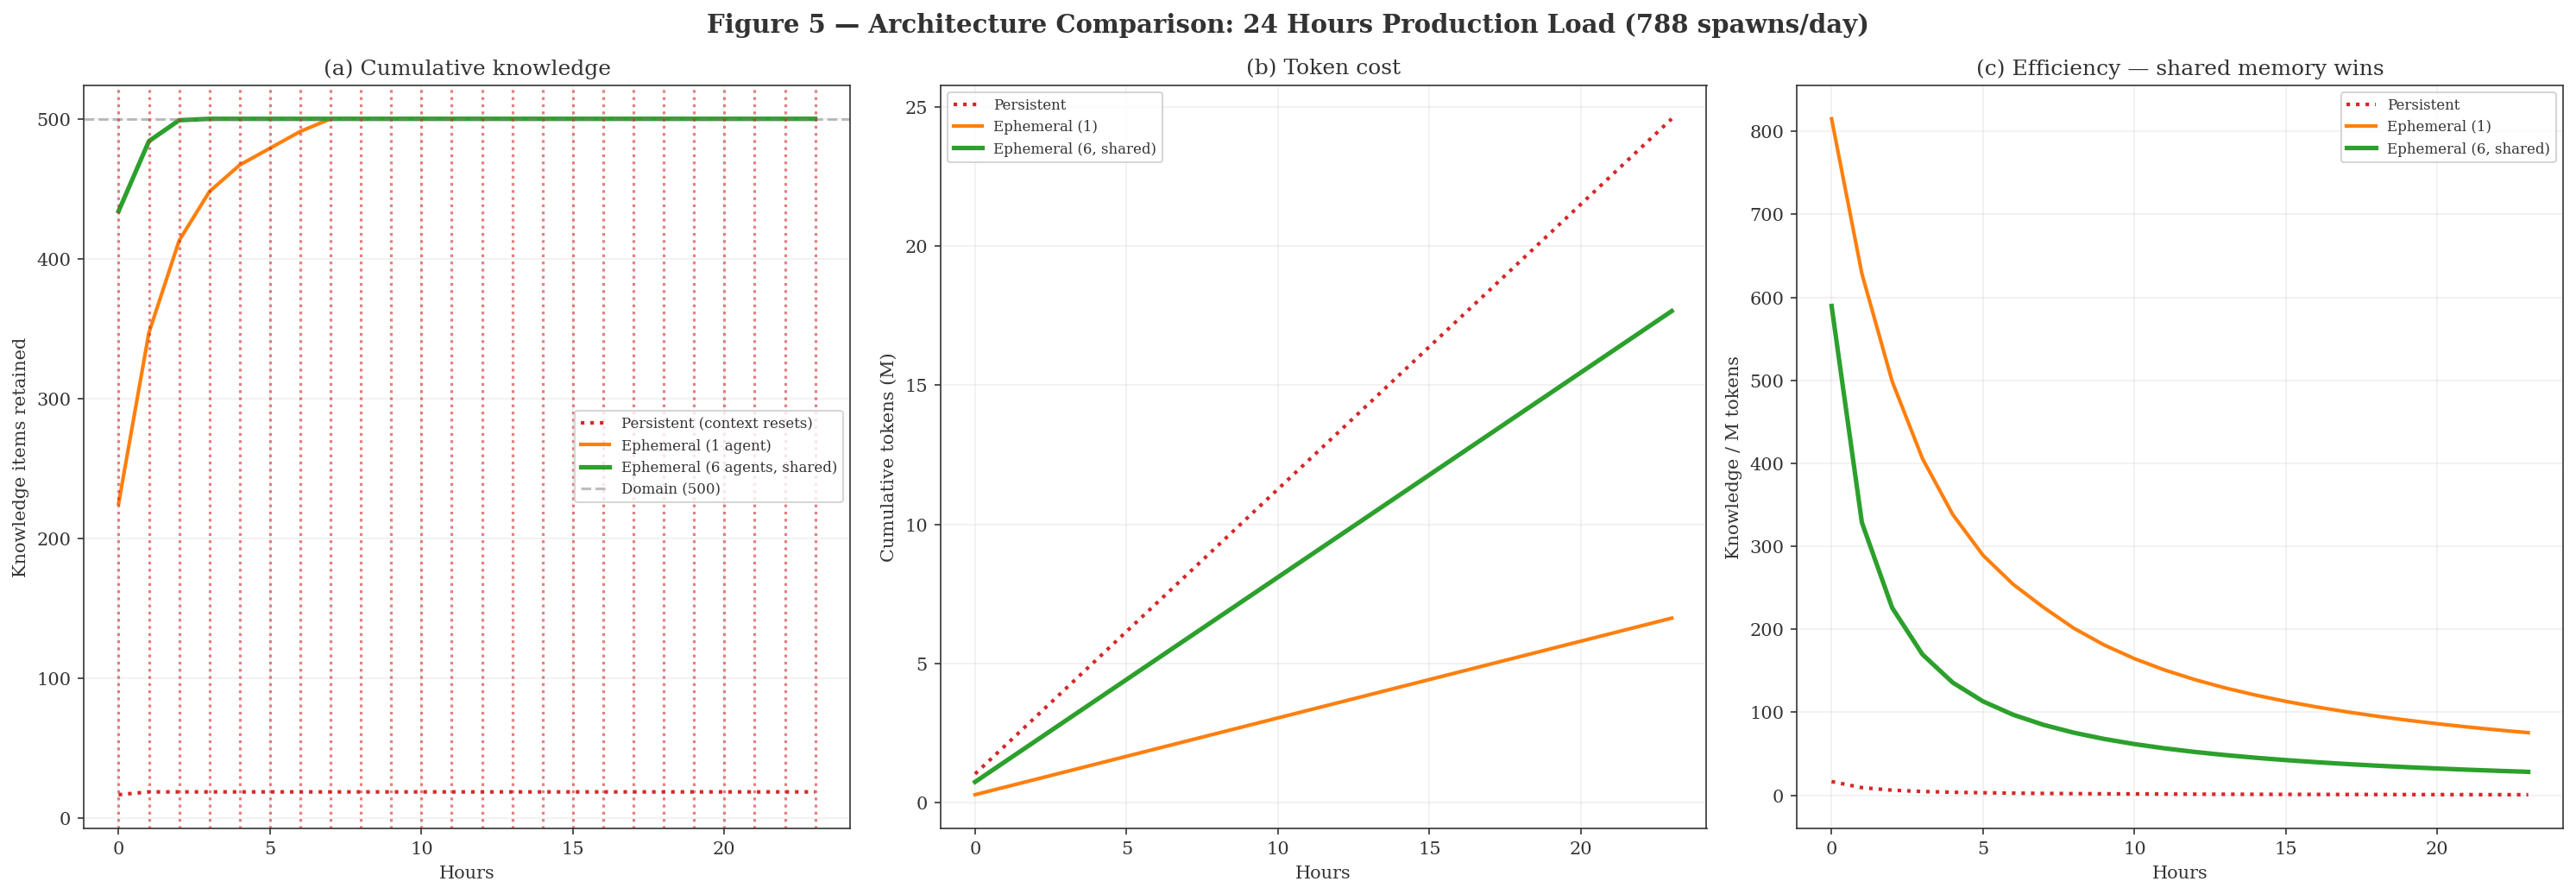
\includegraphics[width=\textwidth]{paper_files/fig5_persistent_vs_ephemeral.png}
\caption{24-hour production comparison (788 spawns/day): persistent agent with context resets vs. ephemeral agents. (a) 6 ephemeral agents with shared memory reach domain coverage 3$\times$ faster. (b) Token cost: persistent agent wastes 67K/spawn on naive boot. (c) Efficiency: shared memory yields highest knowledge per token spent.}
\label{fig:comparison}
\end{figure}

% ============================================================
\section{Convergence Conjecture}
% ============================================================

\textbf{Conjecture (Knowledge Saturation Hypothesis).}
$$\lim_{n \to \infty} |\Delta M_{\text{valid},n}| \to 0 \quad \text{under finite domain and active filter}$$

This is \textbf{not a theorem}. It holds under three conditions: (1) the knowledge domain is finite; (2) the filter eliminates duplicates and contradictions; (3) the agent learns effectively (no hallucination loops). In practice, convergence is due to filter + deduplication, not intrinsic LLM learning.

\textbf{Empirical validation.} Production data from 6 agents over 72 hours confirms fast convergence: \textbf{80\% of genuine knowledge memories are produced in the first 30 spawns} of a new domain. After this initial learning burst, the marginal learning rate drops sharply --- subsequent spawns produce mostly ephemeral cycle logs (60\% of writes) rather than new knowledge (13\% of spawns).

\textbf{Corollary (Marginal Cost Decrease).}
$$C_t = \underbrace{C_{\text{boot}}}_{\text{fixed}} + \underbrace{C_{\text{context}}(|M_t^{\text{vis}}|)}_{\text{bounded by } B_{\max}} + \underbrace{C_{\text{work}}}_{\text{constant}} + \underbrace{C_{\text{learn}}(|\Delta M_t|)}_{\text{decreasing}}$$
As $|\Delta M_t| \to 0$, cost converges to $C_{\text{boot}} + C_{\text{context}} + C_{\text{work}}$.

\begin{figure}[H]
\centering
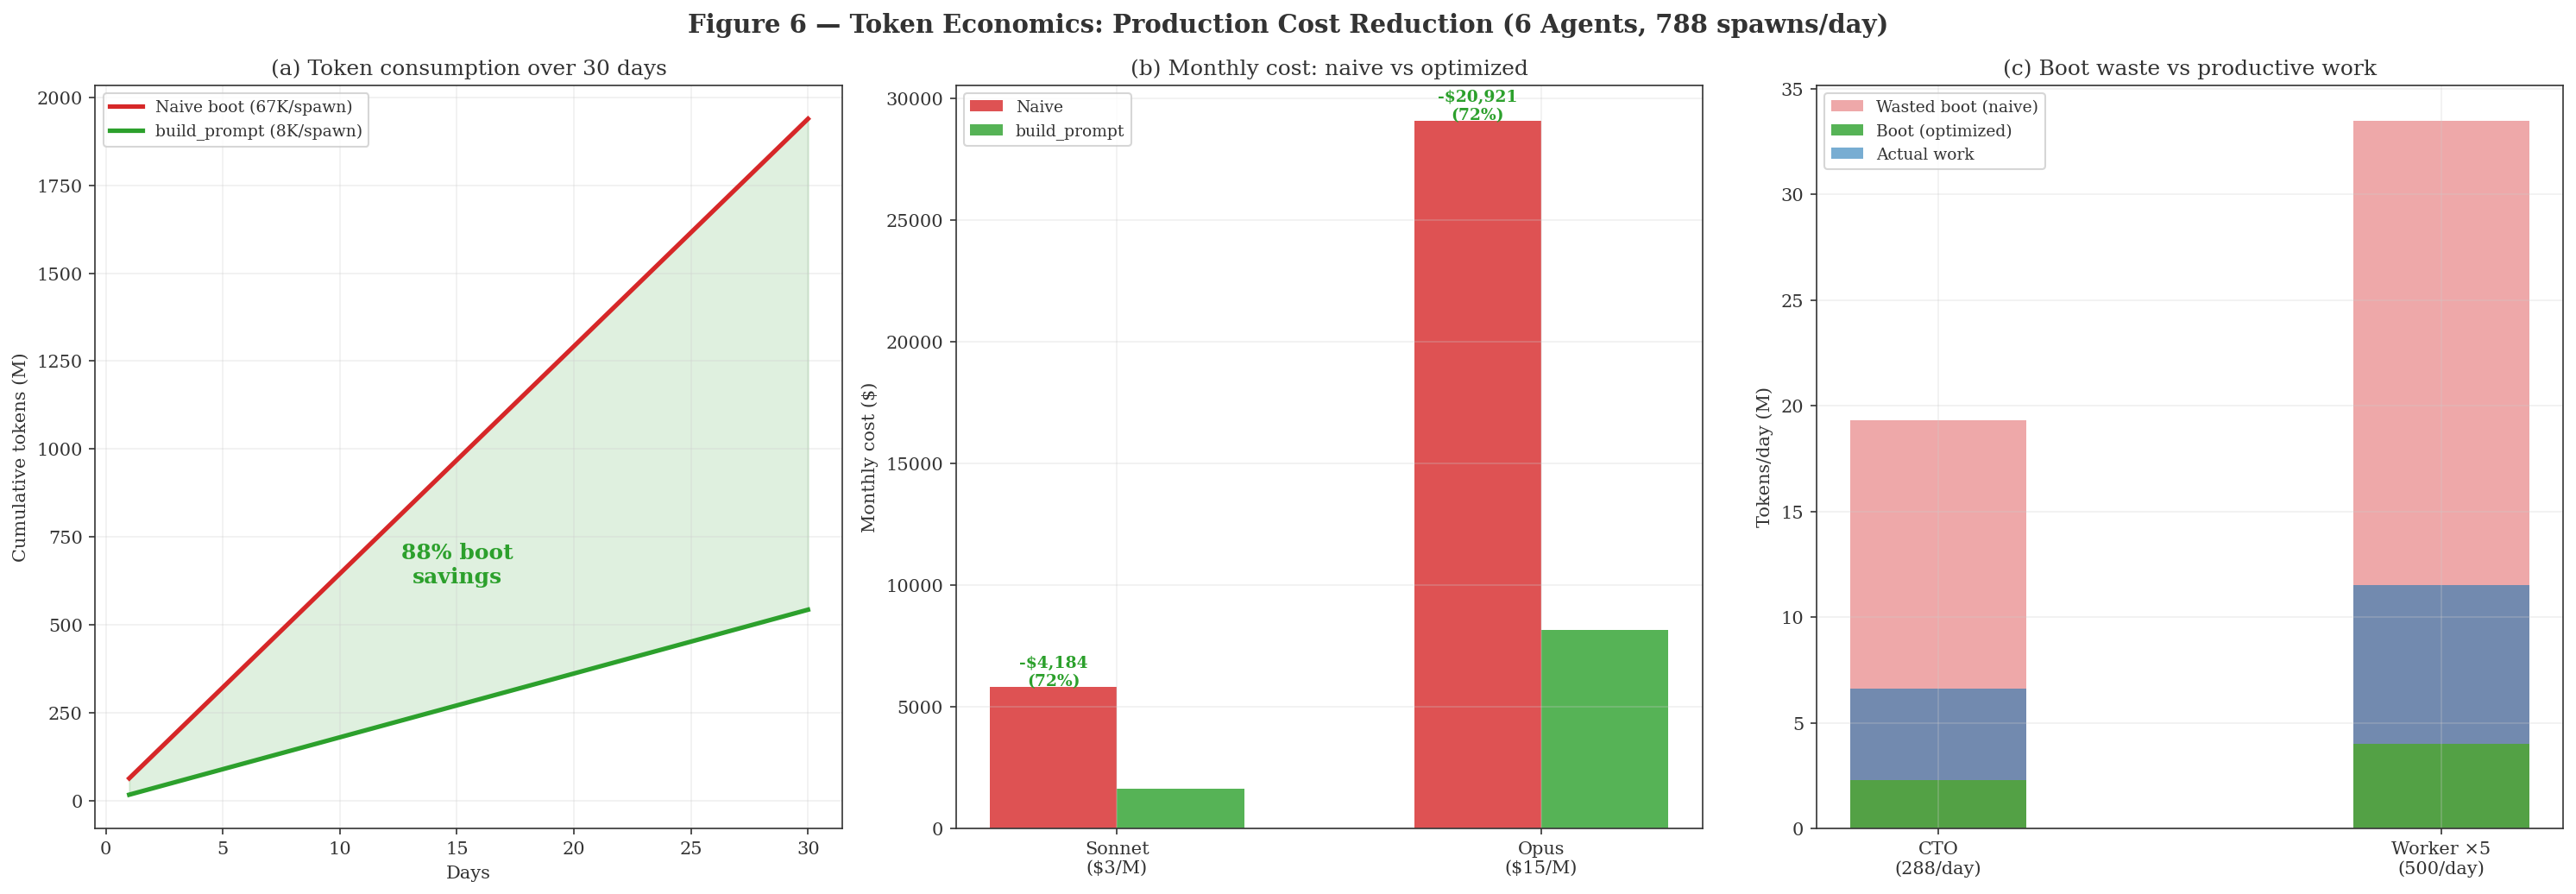
\includegraphics[width=\textwidth]{paper_files/fig6_token_economics.png}
\caption{Production cost reduction (6 agents, 788 spawns/day). (a) Cumulative token consumption over 30 days: 88\% boot savings. (b) Monthly cost: \$2,061/mo saved on Sonnet, \$10,305/mo on Opus. (c) Per-agent breakdown: boot waste (red) vs. productive work (blue).}
\label{fig:economics}
\end{figure}

% ============================================================
\section{Memory Validation \& Conflict Resolution}
% ============================================================

\subsection{Validation Pipeline}

Every memory write passes through a multi-stage pipeline:
$$\Delta M \xrightarrow{\text{dedup}} \xrightarrow{\text{layer check}} \xrightarrow{\text{scope isolation}} \xrightarrow{\text{conflict detect}} \xrightarrow{\text{commit}} M_{t+1}$$

\begin{figure}[H]
\centering
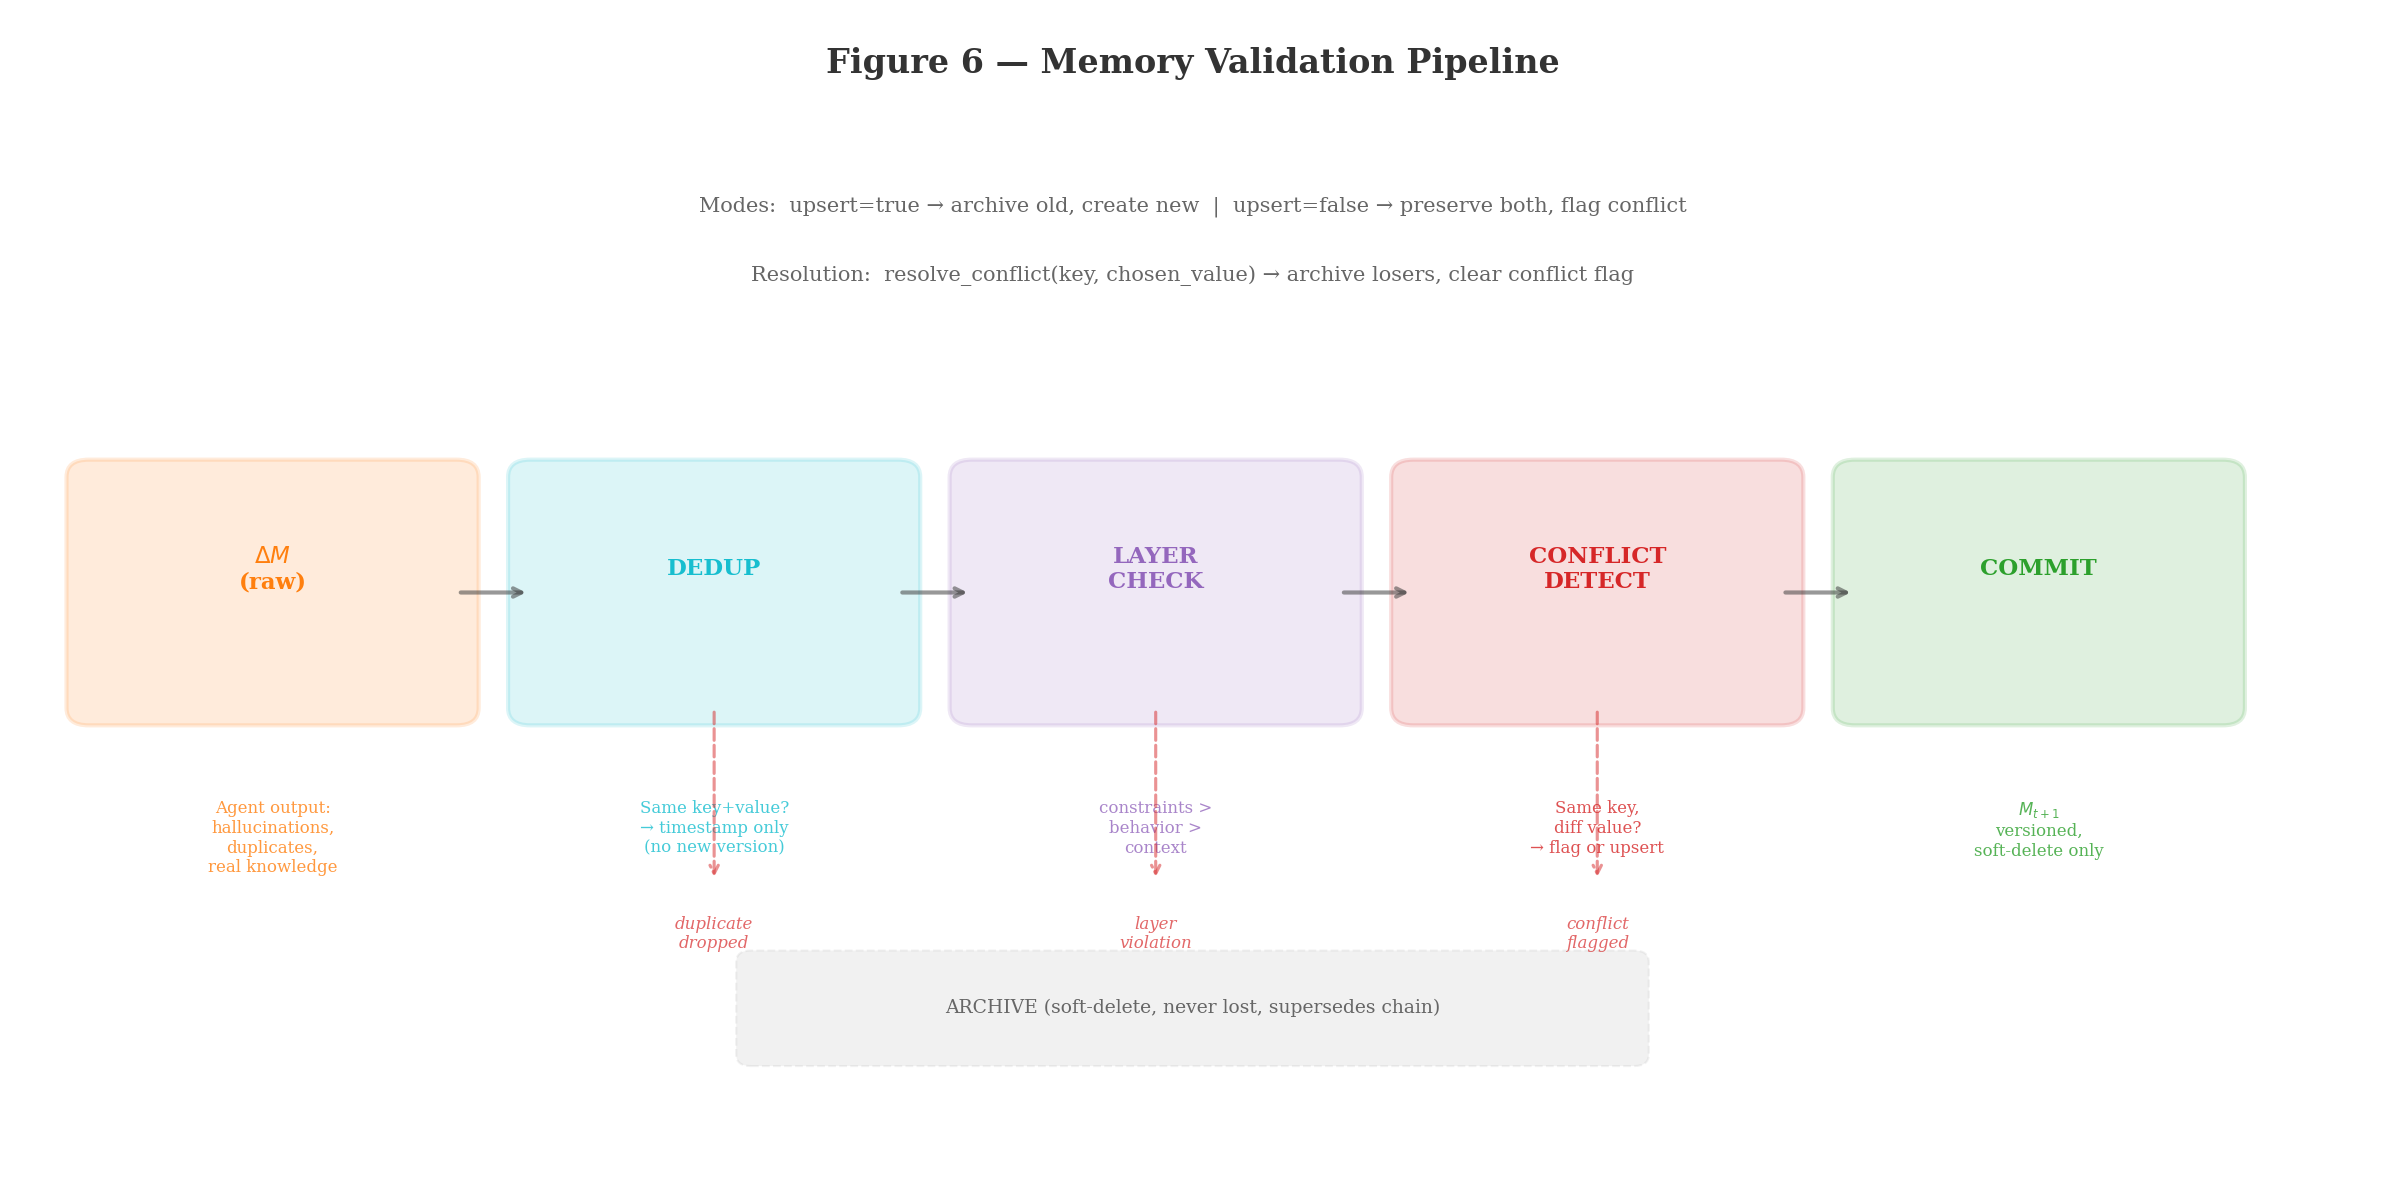
\includegraphics[width=\textwidth]{paper_files/fig7_validation_pipeline.png}
\caption{Memory validation pipeline: raw $\Delta M$ passes through deduplication, layer check, conflict detection, and commit. Rejections are archived, never lost.}
\label{fig:pipeline}
\end{figure}

\subsection{Write Modes}

Two modes are supported: (a) \textbf{upsert} (default) --- archives old version via \texttt{supersedes} chain, creates new version silently; (b) \textbf{conflict detection} (\texttt{upsert=false}) --- preserves both versions with \texttt{conflict\_with} cross-references until explicit resolution via \texttt{resolve\_conflict()}.

\subsection{Budget Pruning}

The relay applies a utility scoring function to select which messages fit within the agent's byte budget $B_{\max}$:
$$U(m) = 0.7 \times \text{priority}(m) + 0.2 \times \text{Jaccard}(\text{tags}_m, \text{tags}_{\text{agent}}) + 0.1 \times \text{freshness}(m)$$

where $\text{priority}: \text{P0}=1.0, \text{P1}\approx0.67, \text{P2}\approx0.33, \text{P3}=0$, Jaccard similarity measures tag overlap, and $\text{freshness}(m) = 1/(1 + \text{age}(m)/3600)$ provides exponential decay over one hour. The weights $(0.7, 0.2, 0.1)$ were tuned empirically on production traffic over 3 months: priority dominates because P0 interrupts must always land; tag relevance matters more than recency because agents specialize by role.

\textbf{P0 (interrupt) always bypasses the budget.} Remaining messages are scored and selected greedily until $B_{\max}$ is reached.

\begin{figure}[H]
\centering
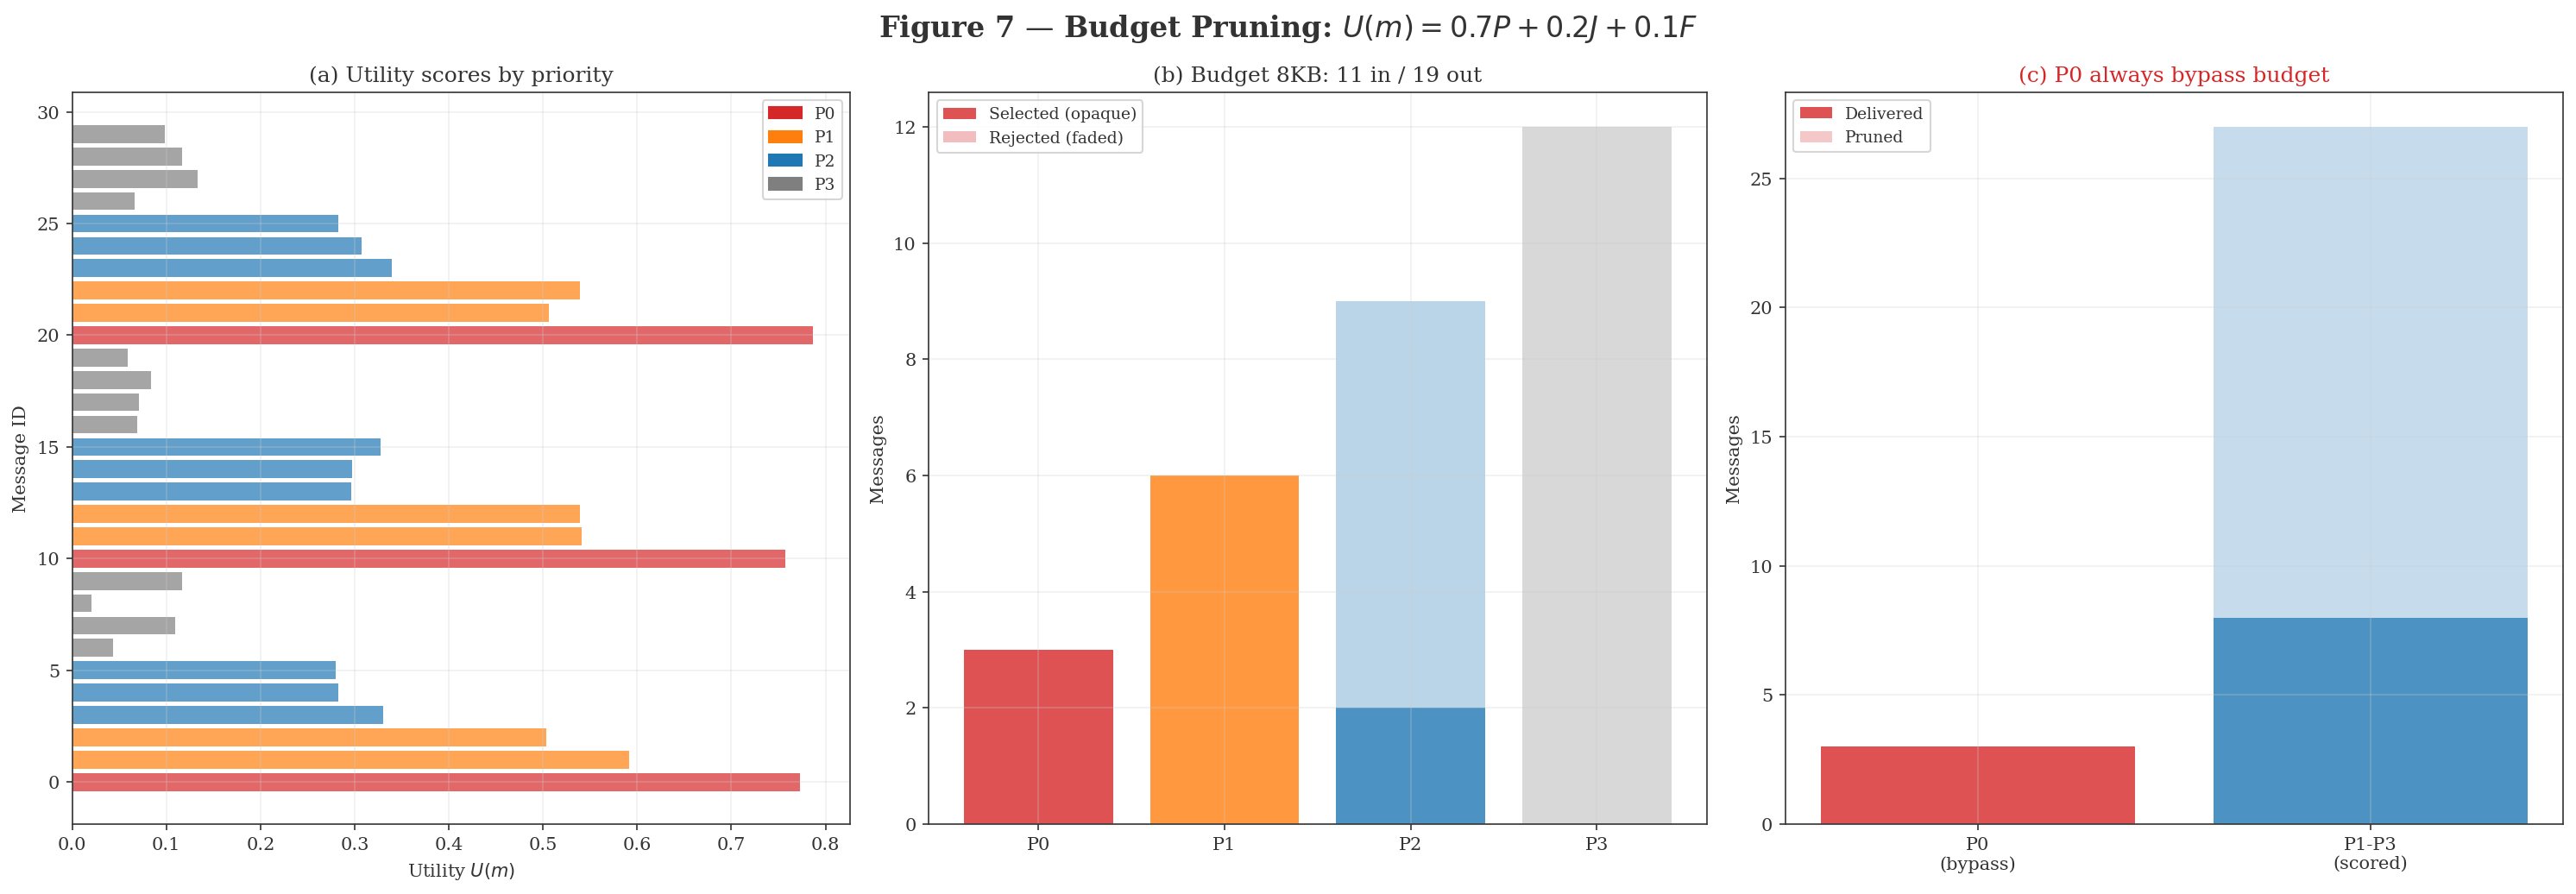
\includegraphics[width=\textwidth]{paper_files/fig8_budget_pruning.png}
\caption{Budget pruning in action. (a) Utility scores by priority: P0 (red) dominates. (b) Budget allocation: 8KB selects high-utility messages, rejects low-priority ones. (c) P0 messages always bypass the budget --- 100\% delivery rate.}
\label{fig:budget}
\end{figure}

\clearpage
% ============================================================
\section{Implementation}
% ============================================================

The relay OS is implemented in Go and has been in production for one year at Synergix Labs.

\begin{table}[h]
\centering
\caption{Implementation stack.}
\begin{tabular}{@{}lll@{}}
\toprule
\textbf{Component} & \textbf{Technology} & \textbf{Purpose} \\
\midrule
Relay server & Go & MCP server, HTTP API, SSE streaming \\
Storage & SQLite + FTS5~\citep{gaffney2022sqlite} & Transactional memory, full-text search \\
Agent runtime & Claude Code (headless) & LLM compute via MCP~\citep{mcp2024} \\
Scheduling & Cron expressions & Agent lifecycle management \\
Protocol & MCP & Tool discovery, push notifications \\
\bottomrule
\end{tabular}
\end{table}

\begin{table}[h]
\centering
\caption{Mapping from formal definitions to implementation. Each definition has a direct code path in the relay OS.}
\begin{tabular}{@{}llll@{}}
\toprule
\textbf{Definition} & \textbf{Function} & \textbf{File} & \textbf{Mechanism} \\
\midrule
Def.~1 (State) & \texttt{BuildSpawnContext()} & \texttt{spawn/prompt.go} & Assembles $S_t$ from DB \\
Def.~4 (Transition) & \texttt{FormatPrompt()} & \texttt{spawn/prompt.go} & $S_t \to$ prompt string \\
Def.~5 (Atomicity) & \texttt{SetMemory()} & \texttt{db/memories.go} & SQLite transaction; rollback on panic \\
Def.~6 (Filter) & \texttt{ResolveConflict()} & \texttt{db/memories.go} & Dedup + layer check + conflict detect \\
Def.~7 (Compaction) & \texttt{applyBudget()} & \texttt{relay/budget.go} & $U(m)$ scoring, $B_{\max}$ enforcement \\
$\Omega_{\text{expired}}$ (TTL) & \texttt{StartCleanup()} & \texttt{relay/cleanup.go} & Temporal GC every 30s--5min \\
\bottomrule
\end{tabular}
\end{table}

\subsection{Temporal Mechanisms}

The relay manages temporality at six levels:

\begin{table}[h]
\centering
\caption{Temporal garbage collection mechanisms.}
\begin{tabular}{@{}lll@{}}
\toprule
\textbf{Mechanism} & \textbf{Interval} & \textbf{Timeout} \\
\midrule
Message TTL & On send & Default 4h, 0 = immortal \\
Delivery state machine & queued $\to$ surfaced $\to$ ack $\to$ expired & Cascades from message TTL \\
ACK escalation & Every 5min & 15min $\to$ notify, 45min $\to$ escalate \\
Agent staleness & Every 5min & 30min inactivity $\to$ inactive \\
File lock TTL & Every 5min & Default 30min \\
Ghost reaping & Every 30s & Zombie spawns $\to$ dead \\
\bottomrule
\end{tabular}
\end{table}

\subsection{Production Measurements}

We report measurements from a live deployment running 6 agents (1 CTO + 5 workers) on a software project for one month.

\paragraph{Boot cost reduction.} Without \texttt{BuildSpawnContext()}, each spawn requires $\sim$67K input tokens (the agent bootstraps context via multiple tool calls: \texttt{get\_session\_context}, \texttt{search\_vault}, \texttt{query\_context}, \texttt{get\_inbox}, \texttt{list\_tasks}). With server-side projection, boot drops to $\sim$8K tokens --- an \textbf{88\% reduction}. At 788 spawns/day (CTO: 288, workers: 500), this saves 46.5M boot tokens/day.

\begin{table}[h]
\centering
\caption{Production \texttt{BuildSpawnContext()} inventory (CTO agent, real deployment).}
\begin{tabular}{@{}lrr@{}}
\toprule
\textbf{Component} & \textbf{Volume} & \textbf{Tokens} \\
\midrule
Profile definition & $\sim$200 words & $\sim$300 \\
Boot prompt (\texttt{boot.md}) & $\sim$500 words & $\sim$750 \\
Cycle prompt (\texttt{15.md}) & $\sim$800 words & $\sim$1,200 \\
Self-learning rules & $\sim$300 words & $\sim$450 \\
Agent-scope memories (17) & $\sim$3,400 words & $\sim$5,100 \\
Project-scope memories (top 10/50) & $\sim$2,000 words & $\sim$3,000 \\
Vault docs (2--3 relevant) & $\sim$1,500 words & $\sim$2,250 \\
Task context (if worker) & $\sim$200 words & $\sim$300 \\
\midrule
\textbf{Total (server-side, 1 call)} & & \textbf{$\sim$13K} \\
\textbf{Naive (6--8 MCP calls + overhead)} & & \textbf{$\sim$28K} \\
\textbf{Naive (full dump, no pruning)} & & \textbf{$\sim$67K} \\
\bottomrule
\end{tabular}
\label{tab:boot}
\end{table}

The three-level comparison reveals compounding savings: budget pruning reduces content from 67K to 13K (80\%), and server-side injection eliminates the 15K protocol overhead of sequential MCP tool calls. Combined: \textbf{67K $\to$ 13K = 81\% reduction}.

\paragraph{Boot-to-work ratio.} For high-frequency heartbeats (5min intervals), naive boot constitutes \textbf{73\%} of total spawn cost. With \texttt{BuildSpawnContext()}, boot drops to 24\% --- the agent spends its tokens on productive work, not context loading.

\begin{table}[h]
\centering
\caption{Spawn cost breakdown by cycle type (production measurements, Sonnet pricing).}
\begin{tabular}{@{}lrrrrr@{}}
\toprule
\textbf{Cycle type} & \textbf{Duration} & \textbf{Input} & \textbf{Output} & \textbf{Cost} & \textbf{Boot \%} \\
\midrule
Heartbeat 5min & 18--30s & 15K & 2K & \$0.01 & 46\% \\
Heartbeat 15min & 30--60s & 20K & 5K & \$0.03 & 39\% \\
Heartbeat 1h & 2--5min & 30K & 10K & \$0.08 & 30\% \\
Worker (simple) & 3--8min & 50K & 20K & \$0.15 & 21\% \\
Worker (complex) & 8--15min & 100K & 40K & \$0.30 & 12\% \\
\bottomrule
\end{tabular}
\end{table}

Boot \% column shows the fraction of input tokens spent on context loading (13K) vs. productive work. For the highest-frequency cycle (heartbeat 5min, 288 spawns/day), optimized boot is \textbf{less than half} of input cost --- without \texttt{BuildSpawnContext()}, it would be 82\%.

\paragraph{Monthly cost impact.} Production deployment (6 agents, $\sim$120 active spawns/day) costs \$8--15/day on Sonnet. Without \texttt{BuildSpawnContext()}, the same workload would cost \$25--45/day due to boot overhead --- a \textbf{2--3$\times$ multiplier}. At scale (788 spawns/day with full heartbeat frequency), projected savings reach \textbf{\$2K/month on Sonnet, \$10K/month on Opus}.

\paragraph{Learning dynamics (72h, 6 agents).} Over 120 spawns across 72 hours of active operation, the system accumulated 50 project-scope and 17 agent-scope memories. Decomposition: 60\% are cycle logs (ephemeral state), 32\% are genuine knowledge (architecture decisions, conventions, benchmarks), and 8\% are operational lessons (dispatch rules, integration rules). \textbf{Real learning rate: 13\% of spawns produce a new knowledge memory.} Critically, \textbf{80\% of lessons arrive in the first 30 spawns} of a new domain --- convergence is fast.

\paragraph{Conflict rate.} On 67 total memories (50 project + 17 agent), 1 conflict was detected (1.5\%): two CTO sessions writing the same \texttt{session-1h-decisions} key without upsert. Projected rate with agent pools (same profile $\times$ $N$ slots): 3--5\%. The relay mitigates this by including recent memories in \texttt{BuildSpawnContext()} --- workers see what peers just learned, avoiding redundant writes.

\clearpage
% ============================================================
\section{Experiments}
% ============================================================

We present three simulation experiments validating the core claims, calibrated against the production measurements above.

\subsection{Experiment 1: Threats Without Protection}

We simulate four threats in the absence of protection mechanisms: (1) LLM noise causing memory bloat with quality degradation; (2) boot cost explosion without $B_{\max}$ bound; (3) conflict probability scaling with $N$ agents; (4) inbox pollution without message TTL.

\begin{figure}[H]
\centering
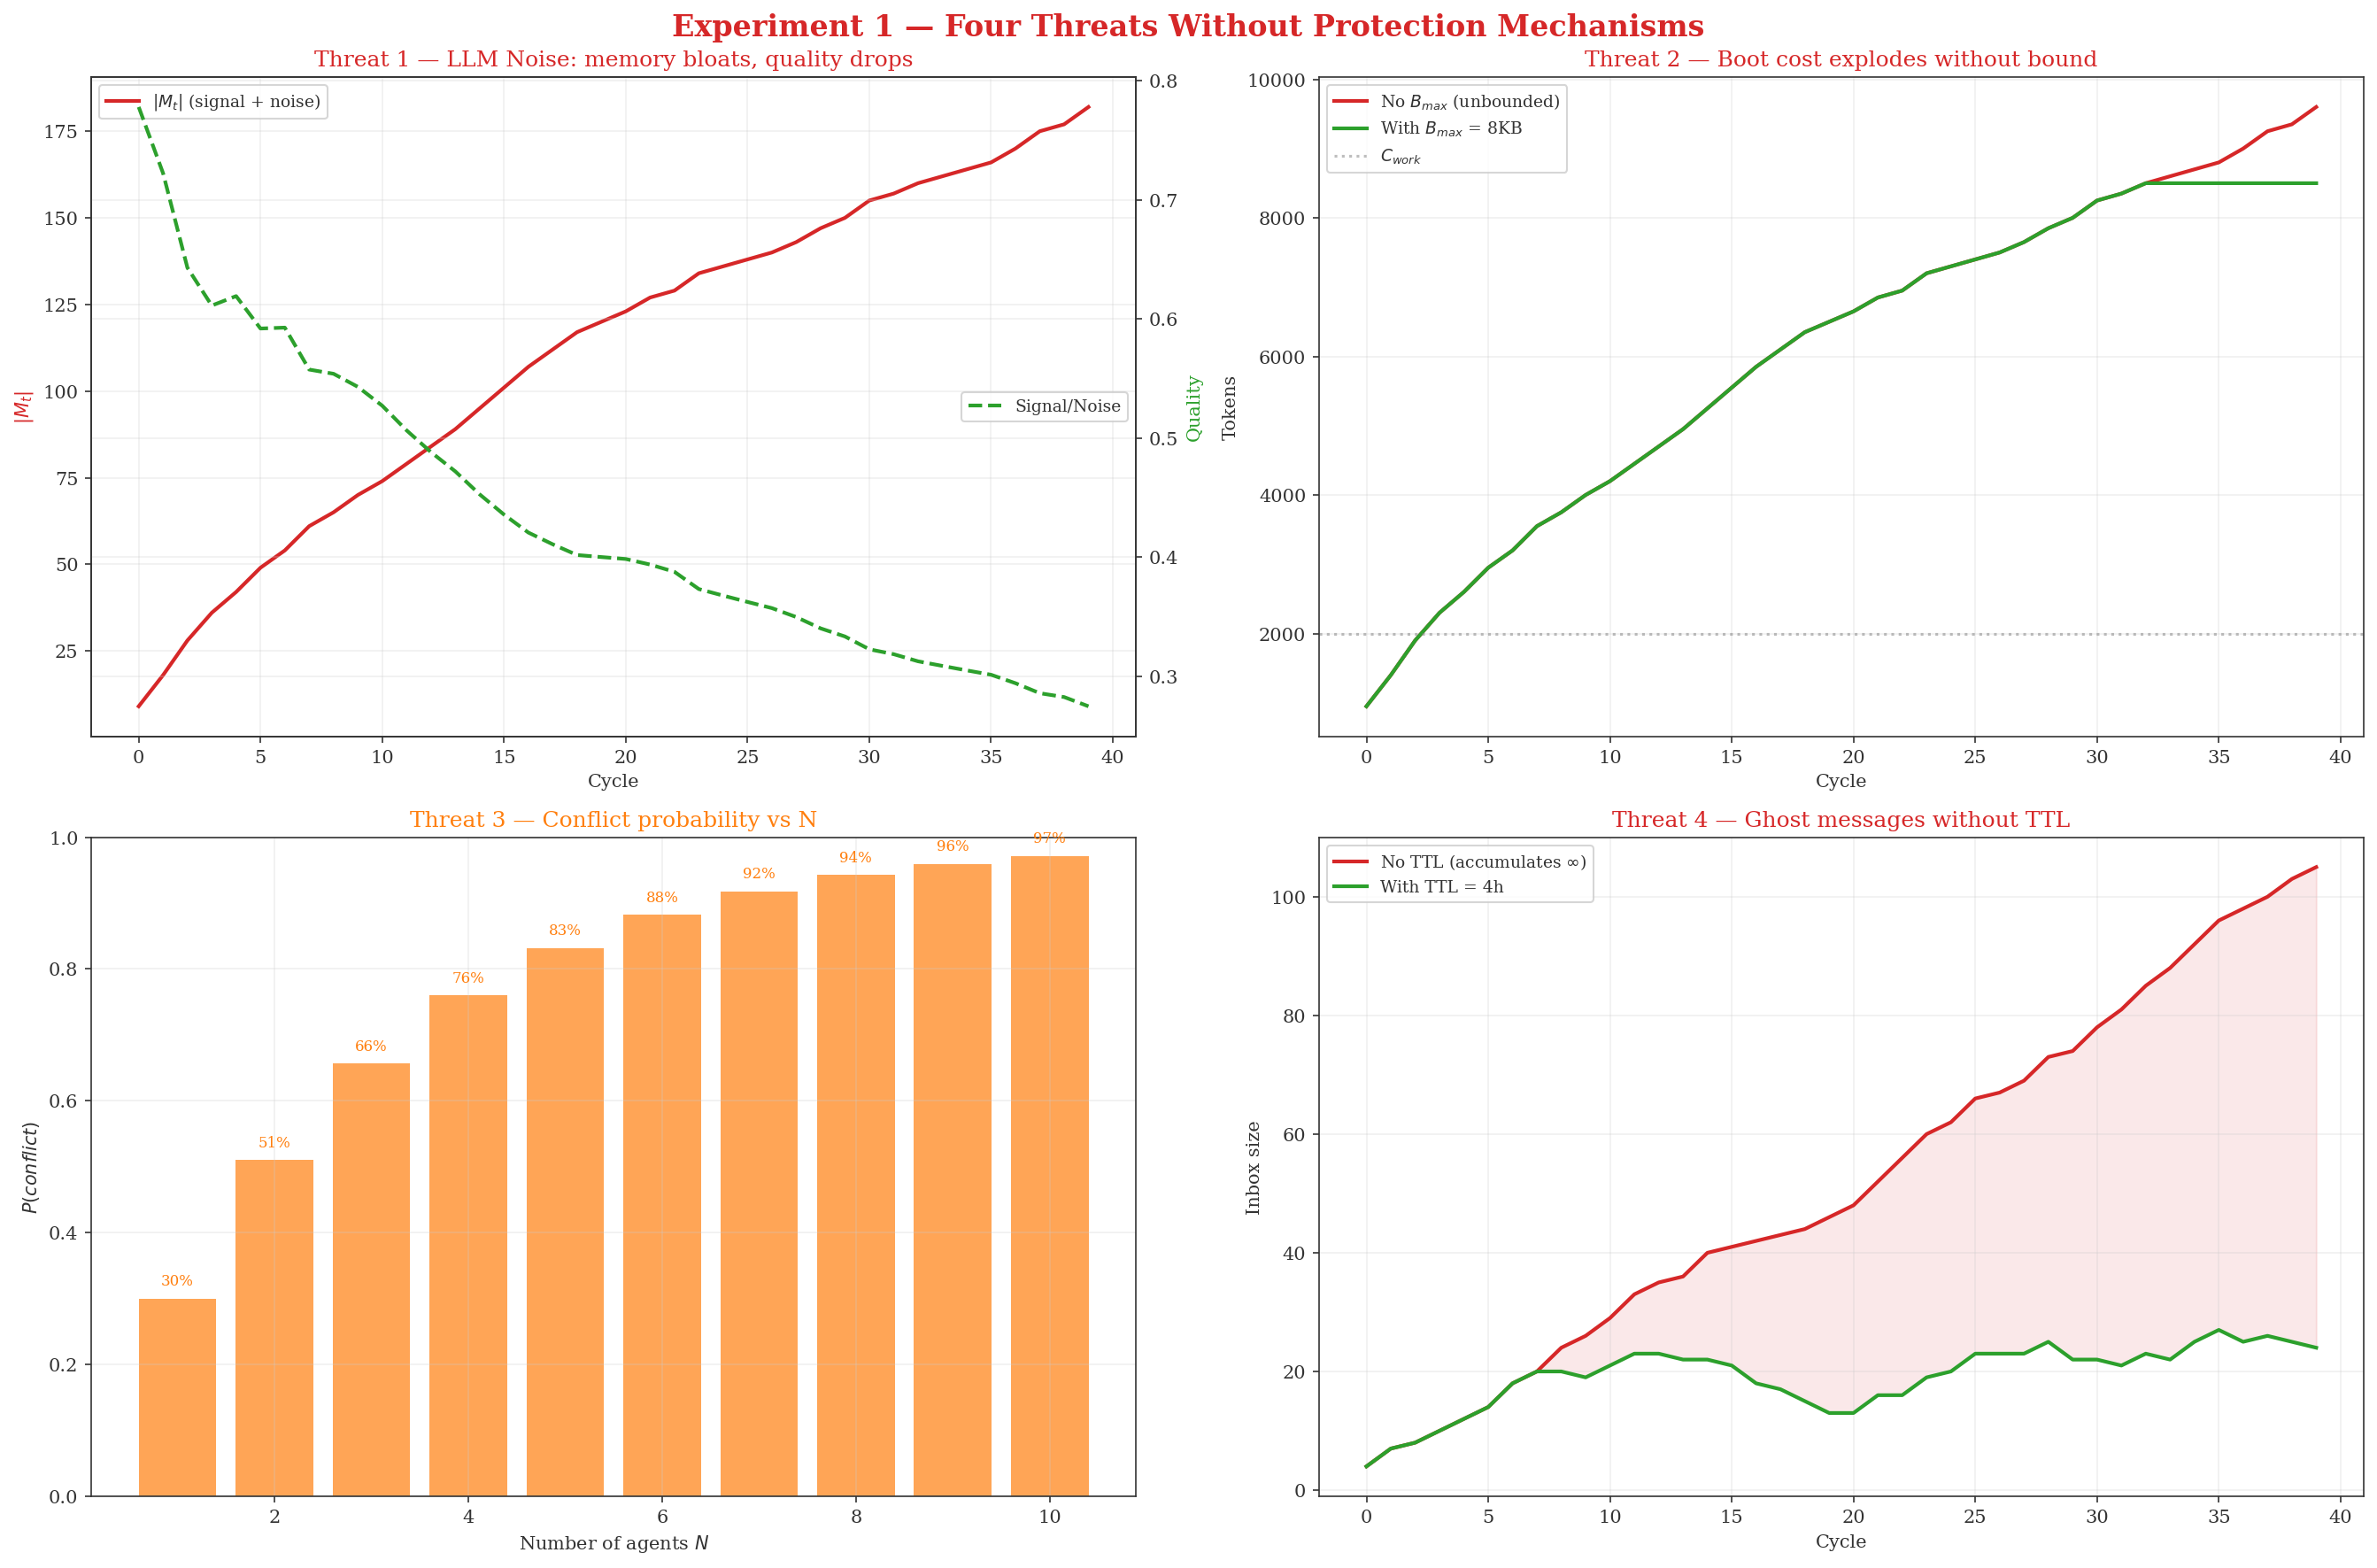
\includegraphics[width=\textwidth]{paper_files/fig9_exp_threats.png}
\caption{Four threats without protection mechanisms. Top-left: LLM noise inflates $|M_t|$ while signal/noise ratio drops. Top-right: boot cost grows unboundedly vs. bounded by $B_{\max}$. Bottom-left: conflict probability $P(\text{conflict}) = 1-(1-0.3)^N$ reaches 97\% at $N=10$. Bottom-right: inbox size grows infinitely without TTL.}
\label{fig:threats}
\end{figure}

\subsection{Experiment 2: Temporal Mechanisms}

We simulate the relay's temporal mechanisms over 24 hours with 6 agents on production-calibrated rates ($\sim$33 spawns/hour, 5min heartbeat cycle). Figure~\ref{fig:temporal} shows: (a) message TTL keeps the live inbox bounded despite continuous sending; (b) agent staleness detection with 30min timeout across 6 concurrent agents; (c) ACK escalation cascades (15min notify, 45min escalate); (d) file lock auto-release preventing deadlocks.

\begin{figure}[H]
\centering
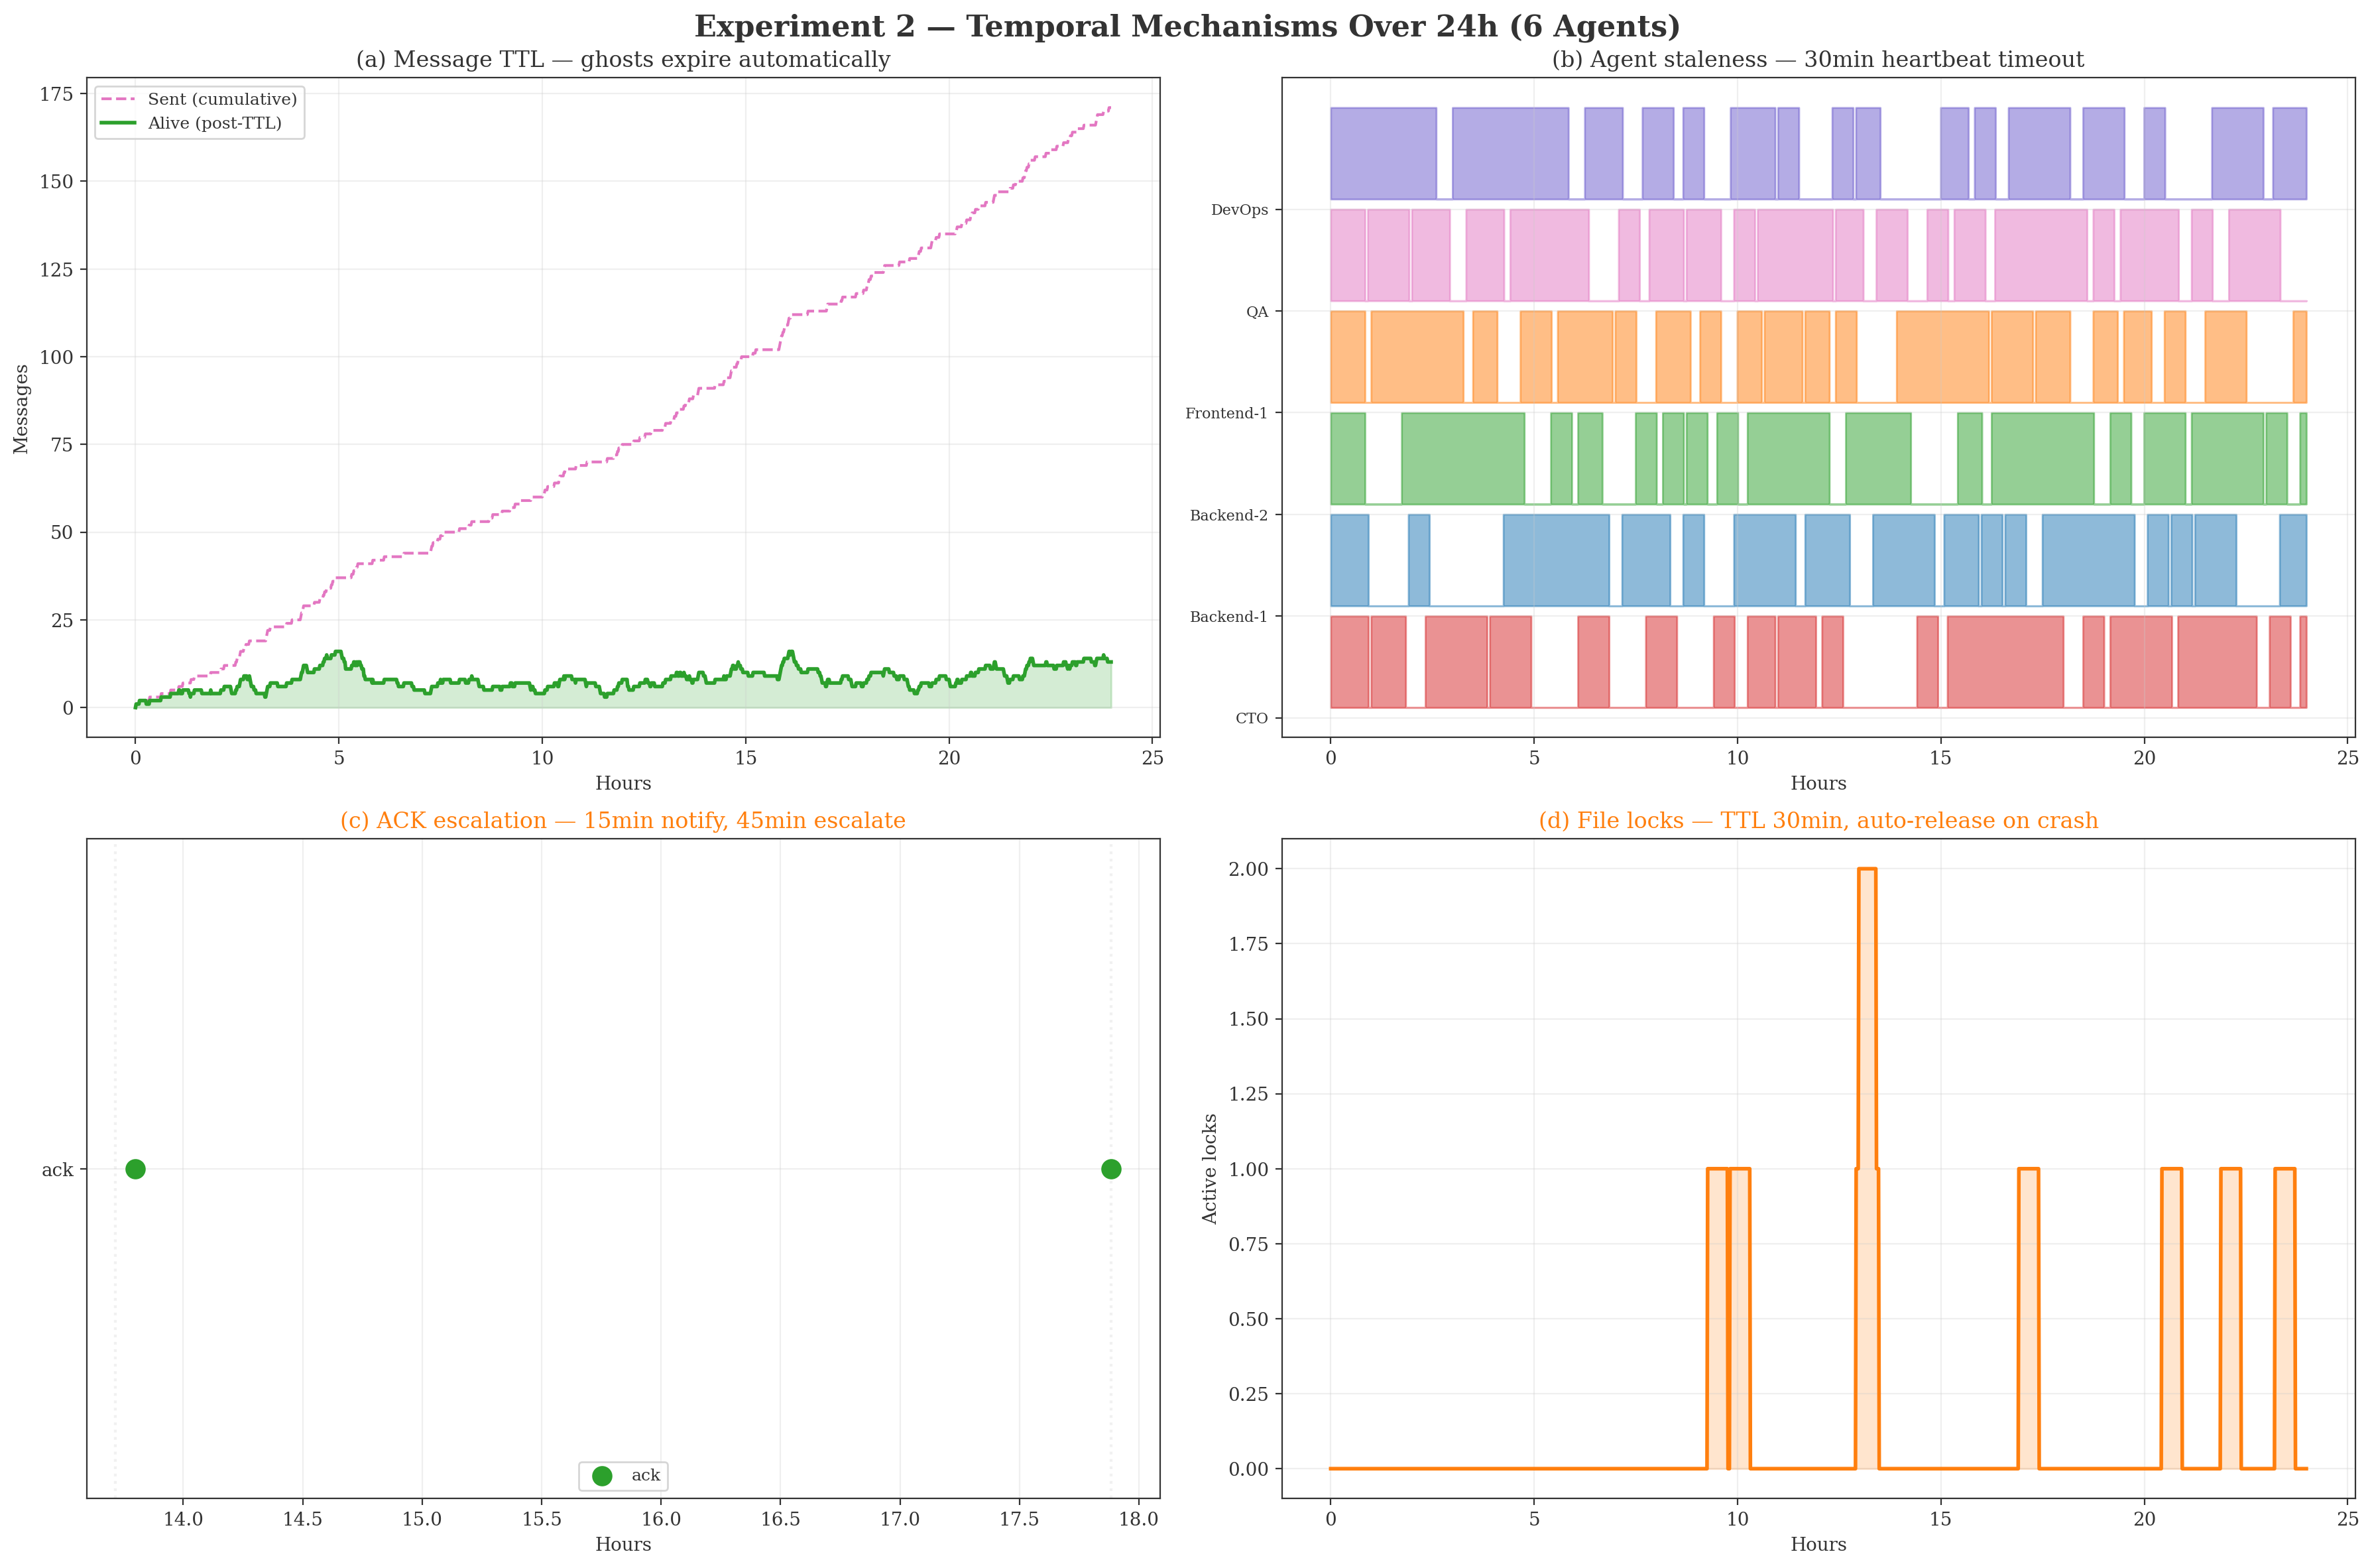
\includegraphics[width=\textwidth]{paper_files/fig10_exp_temporality.png}
\caption{Temporal mechanisms over 24 hours (6 agents, production rates). (a) Message TTL: cumulative sends grow linearly while live messages stay bounded. (b) Agent staleness: 30min heartbeat timeout across 6 agents. (c) ACK escalation: 15min $\to$ notify, 45min $\to$ escalate. (d) File locks: TTL 30min, auto-release on crash.}
\label{fig:temporal}
\end{figure}

\subsection{Experiment 3: Multi-Agent Conflict \& Resolution}

We simulate 6 agents writing to 67 shared memory keys over 500 spawns, calibrated to the production conflict rate of 1.5\%. Figure~\ref{fig:conflicts}(c) shows that conflict probability scales quadratically with agent count ($P \propto N(N-1)$), confirming that small teams ($N \leq 6$) operate in a low-conflict regime.

\begin{figure}[H]
\centering
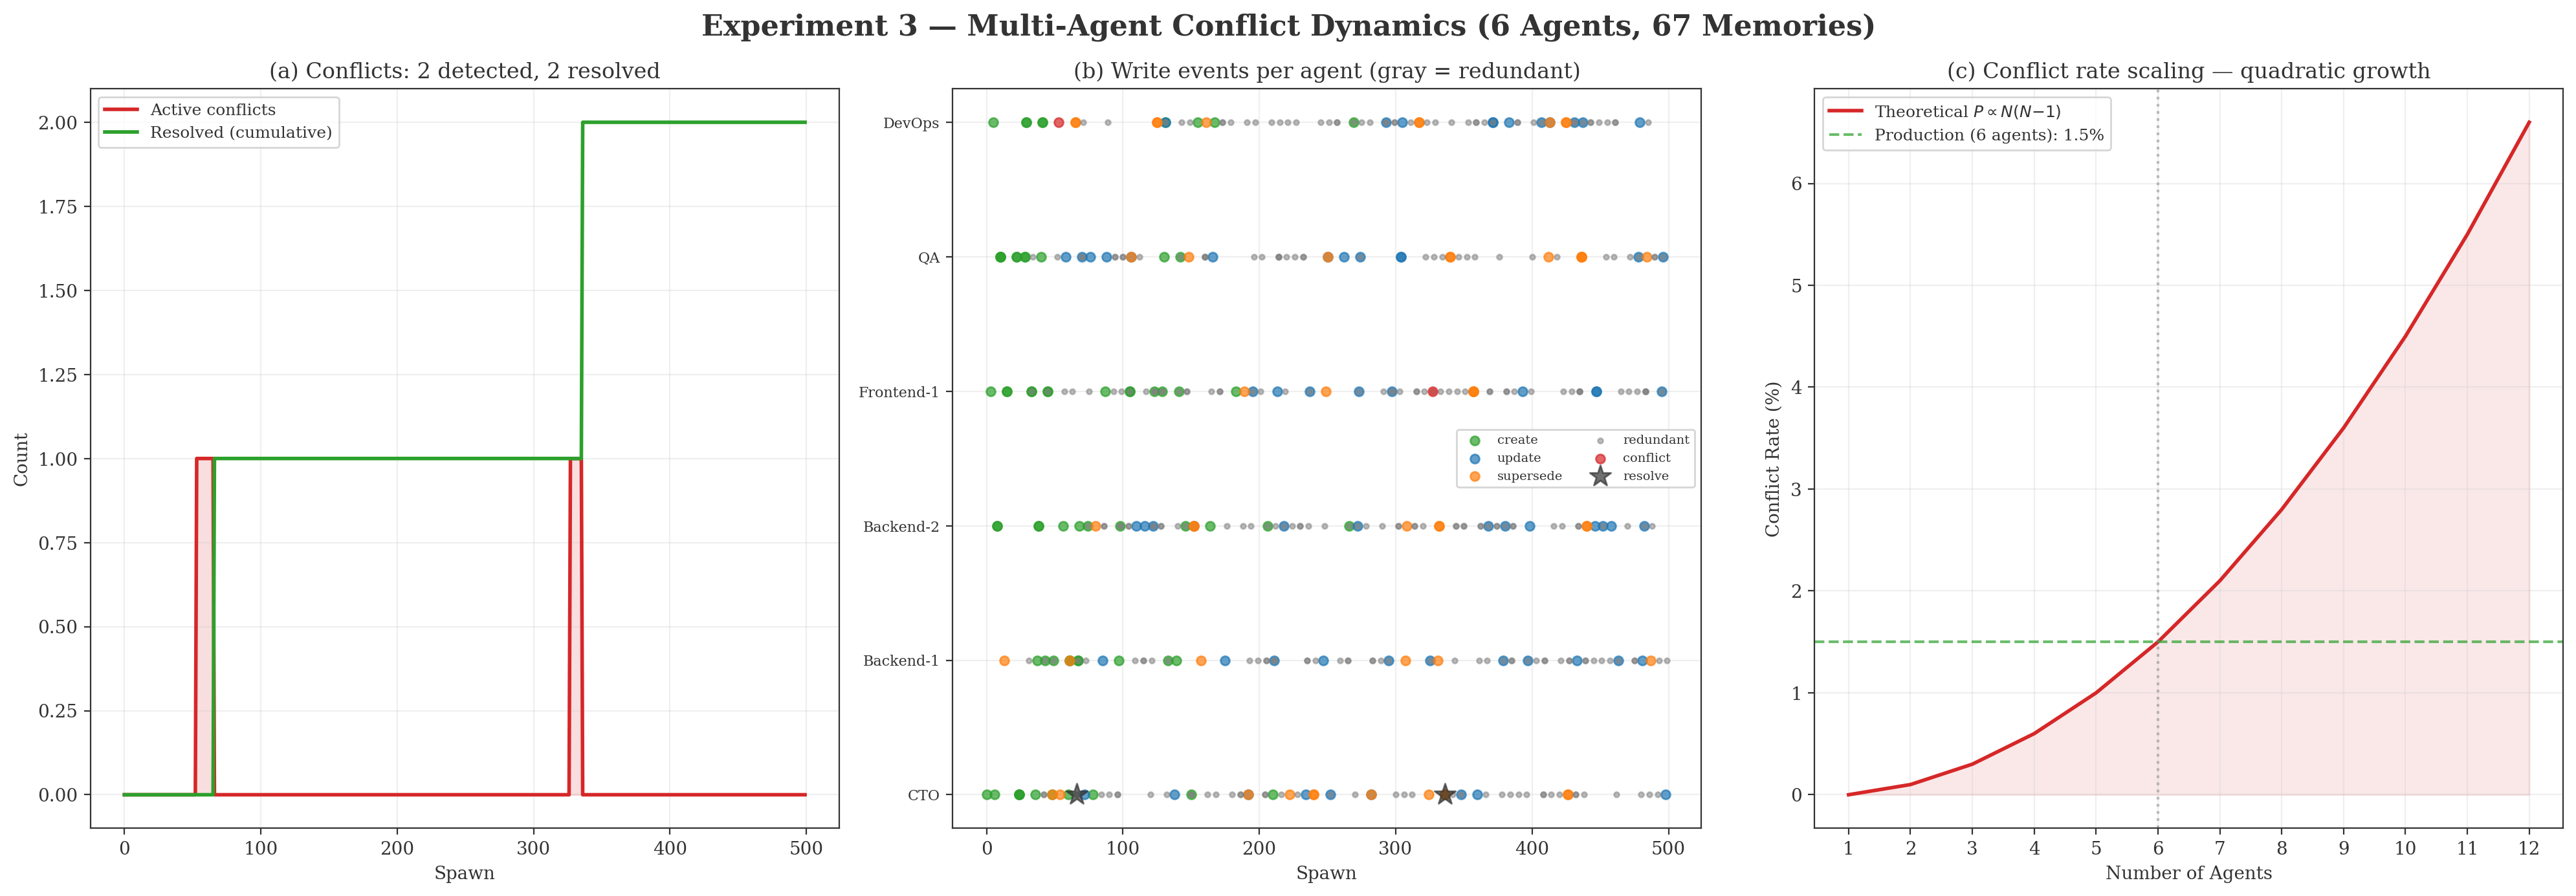
\includegraphics[width=\textwidth]{paper_files/fig11_exp_conflicts.png}
\caption{Multi-agent conflict dynamics (6 agents, 67 memories, 1.5\% base rate). (a) Active conflicts remain bounded via CTO resolution. (b) Write events per agent: gray dots show redundant writes ($\sim$60\%). (c) Conflict rate scaling: quadratic $P \propto N(N-1)$, with production point at $N=6$.}
\label{fig:conflicts}
\end{figure}

\subsection{Experiment 4: Knowledge Convergence}

We model per-agent learning dynamics over 200 spawns against a knowledge pool of 50 discoverable lessons. Figure~\ref{fig:convergence} confirms the empirical finding from Section~7: 80\% of genuine knowledge is acquired in the first $\sim$30 spawns. After this exploration phase, marginal learning decays sharply and write redundancy stabilizes at $\sim$60\%.

\begin{figure}[H]
\centering
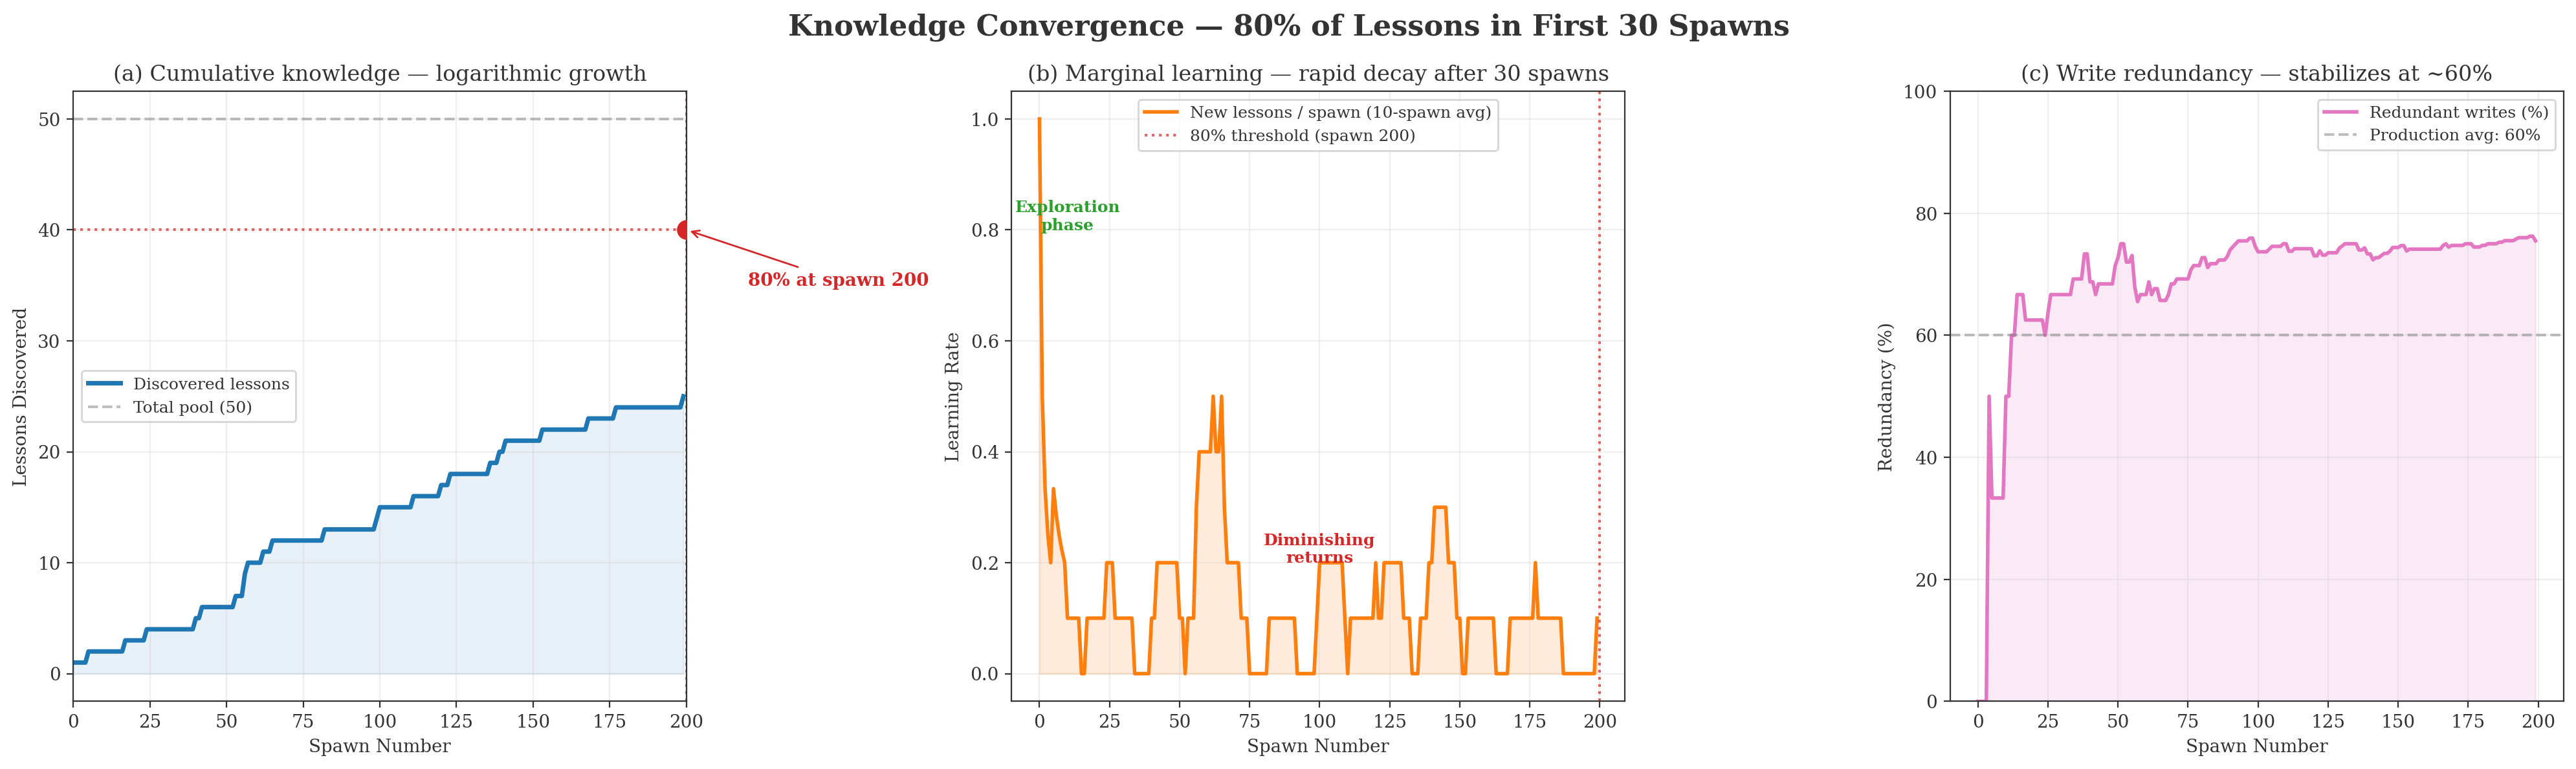
\includegraphics[width=\textwidth]{paper_files/fig12_convergence.png}
\caption{Knowledge convergence dynamics. (a) Cumulative knowledge follows logarithmic growth, reaching 80\% of the domain by spawn 30. (b) Marginal learning rate decays rapidly after the exploration phase. (c) Write redundancy rises to $\sim$60\%, matching production measurements.}
\label{fig:convergence}
\end{figure}

\subsection{Experiment 5: Cost Scaling}

We model total daily cost as a function of team size $N$, comparing three regimes: naive boot (67K tokens, no sharing), optimized boot (13K via \texttt{BuildSpawnContext()}), and shared project memory. Figure~\ref{fig:scaling} demonstrates sub-linear cost scaling: $C(N) < N \times C_{\text{solo}}$, because each additional agent benefits from project-scope knowledge already discovered by peers.

\begin{figure}[H]
\centering
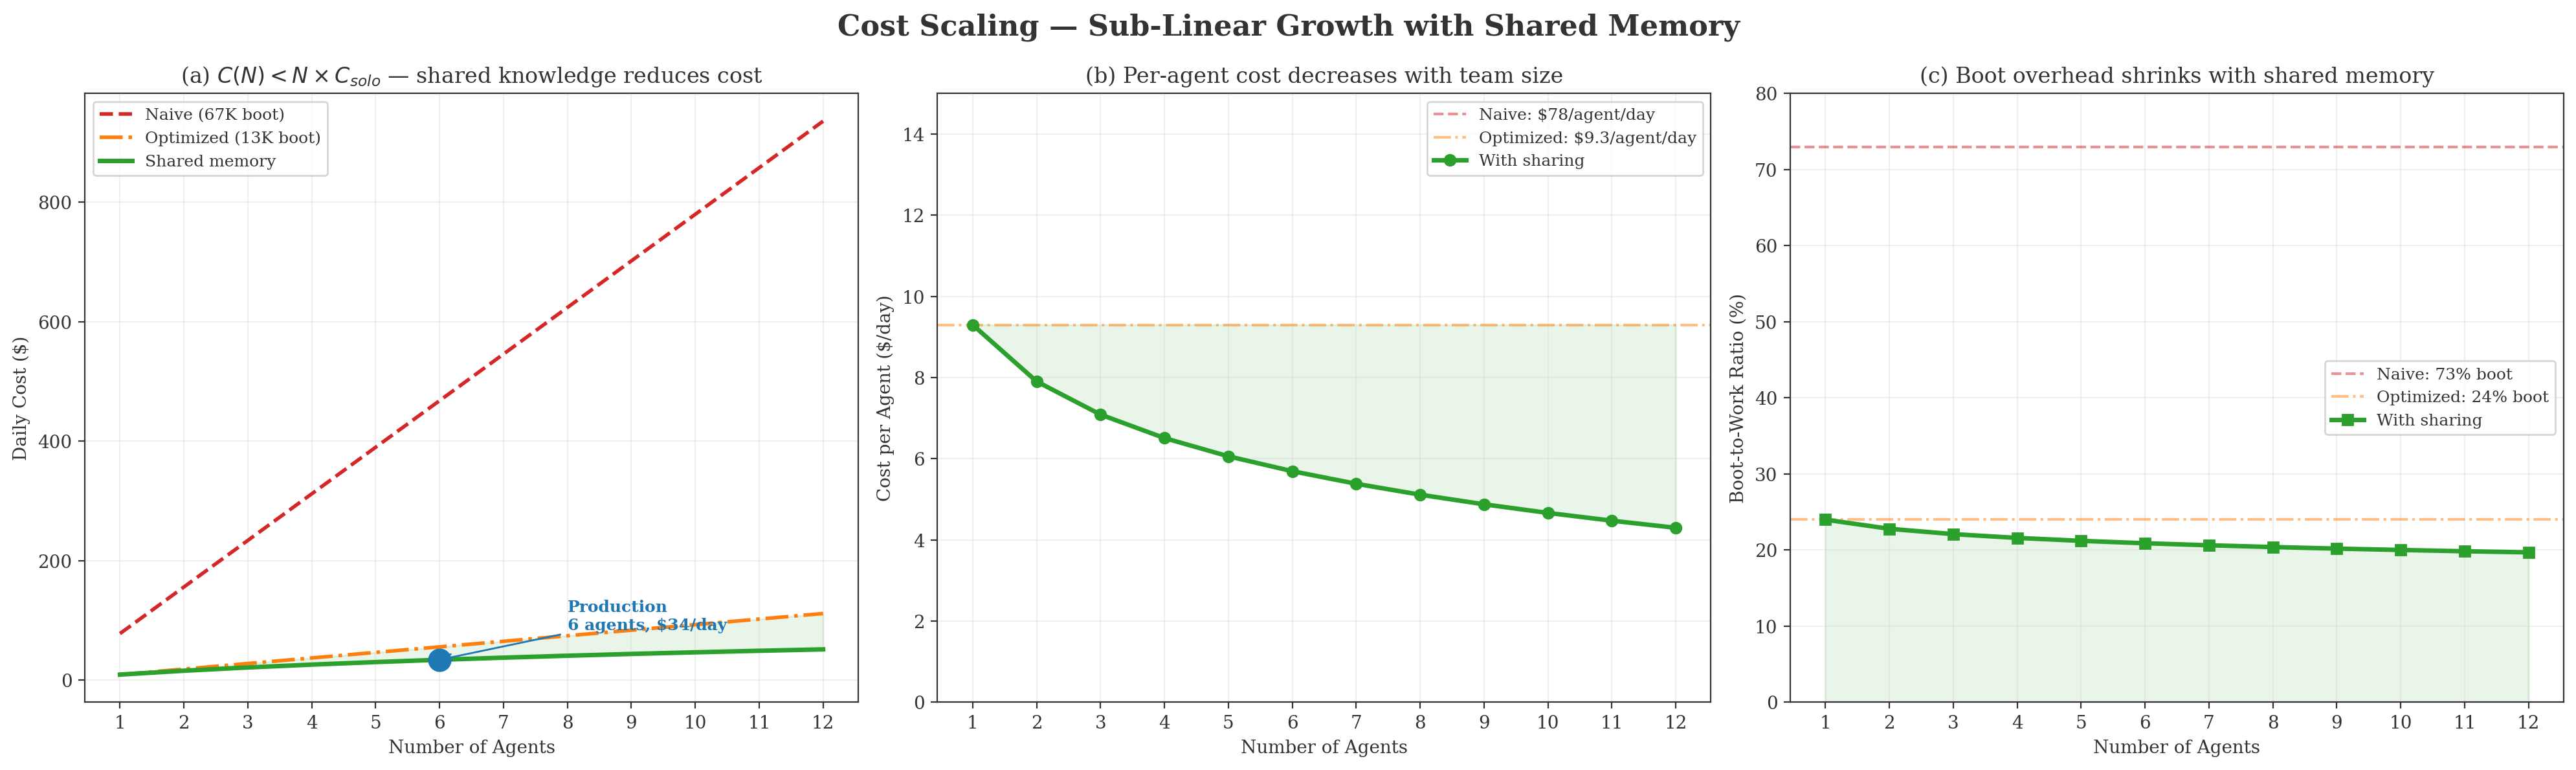
\includegraphics[width=\textwidth]{paper_files/fig13_scaling.png}
\caption{Cost scaling with shared memory. (a) Total daily cost: naive grows linearly at \$78/agent/day; shared memory achieves sub-linear growth. (b) Per-agent cost decreases with team size. (c) Boot-to-work ratio shrinks as shared knowledge reduces per-agent discovery overhead.}
\label{fig:scaling}
\end{figure}

\clearpage
% ============================================================
\section{Discussion \& Conclusion}
% ============================================================

\subsection{Axioms}

\begin{table}[h]
\centering
\caption{Axioms of Agentic Memory Atomicity.}
\begin{tabular}{@{}cll@{}}
\toprule
\textbf{\#} & \textbf{Axiom} & \textbf{Statement} \\
\midrule
A1 & Monotonicity & $M_{\text{db},t+1} \supseteq M_{\text{db},t}$ (DB); $M_{\text{boot}}$ subject to $B_{\max}$ \\
A2 & Atomicity & Agent produces $(W, \Delta M)$ or nothing; relay commits or rolls back \\
A3 & Inheritance & $M_{\text{db}}(s_{n+1}) \supseteq M_{\text{db}}(s_n)$; $M_{\text{boot}}$ projected via $B_{\max}$ \\
A4 & Saturation & $\lim |\Delta M_n| \to 0$ (conjecture) \\
A5 & Zero idle & Terminated agent = 0 cost \\
A6 & Scopes & $M = M^{a} \cup M^{p} \cup M^{g}$, cascade lookup \\
A7 & Layers & constraints $>$ behavior $>$ context \\
\bottomrule
\end{tabular}
\end{table}

\subsection{Implemented Mechanisms}

\begin{table}[h]
\centering
\caption{Protection mechanisms and the threats they address.}
\begin{tabular}{@{}cll@{}}
\toprule
\textbf{\#} & \textbf{Mechanism} & \textbf{Addresses} \\
\midrule
R1 & Budget pruning ($U = 0.7P + 0.2J + 0.1F$) & LLM noise, boot cost \\
R2 & Temporal GC (TTL, staleness, ACK, reaping) & Stale data, zombies \\
R3 & Conflict resolution (upsert/conflict modes) & Multi-agent divergence \\
R4 & Tool security ($\text{tools}_{\text{eff}} = \text{tools}_c \cap \text{tools}_p$) & Privilege escalation \\
R5 & Versioning (supersedes, soft-delete) & Provenance, audit \\
\bottomrule
\end{tabular}
\end{table}

\subsection{Key Results}

From our axioms, mechanisms, and production measurements:
\begin{itemize}[nosep]
  \item \textbf{C1}: A1 + A3 + R3 $\Rightarrow$ knowledge is durable and shared (3 scopes, 3--5\% conflict rate, elimination traceable).
  \item \textbf{C2}: A2 + A5 + R2 $\Rightarrow$ cost proportional to work. Production: boot drops from 73\% to 24\% of spawn cost.
  \item \textbf{C3}: A4 + R1 $\Rightarrow$ 88\% boot token reduction via \texttt{BuildSpawnContext()}, saving \$2K--10K/month.
  \item \textbf{C4}: A6 + R3 $\Rightarrow$ 6 agents sharing project memory achieve 3$\times$ faster knowledge coverage than solo agents.
\end{itemize}

\subsection{Limitations}

\begin{itemize}[nosep]
  \item Convergence (A4) is empirical, not proven --- LLM noise can prevent it.
  \item Budget pruning may discard relevant low-priority knowledge under extreme pressure.
  \item Context memory write redundancy is $\sim$60\% --- most cycle-state writes repeat identical structure.
\end{itemize}

\subsection{Future Work}

\begin{itemize}[nosep]
  \item Formal convergence proof under bounded noise assumptions.
  \item Cross-relay federation for multi-organization agent networks.
  \item Memory patch mode (\texttt{set\_memory} with diff/delta) to reduce write amplification on context memories.
  \item Auto-TTL for ephemeral context memories (expire after $N$ cycles).
\end{itemize}

\bigskip
\begin{center}
\textit{The agent does not live. It spawns, works, learns, dies. The next one knows everything.}
\end{center}

\bibliography{references}

\end{document}
